\chapter{Set theory}
\url{math.colorado.edu/~monkd}

\url{philsci-archive.pitt.edu/1372/1/SetClassCat.PDF}

\url{https://mathoverflow.net/questions/22635/can-we-prove-set-theory-is-consistent}

Rethinking set theory - Leinster




\section{Some initial ideas}
\begin{enumerate}
\item Sets are defined by what is in them (extensionality);
\item Sets can be created by specifying a condition: for any definite condition $P$ there is a set
\[ A = \{x\;|\;P(x)\} \]
defined by $x\in A \iff P(x)$. This is de \udef{general comprehension principle}.
\end{enumerate}
\subsection{Russell's paradox}
Russell showed that the general comprehension principle cannot be valid. Consider
\[ R = \{x\;|\; x\;\text{is a set and}\;x\notin x\}. \]
Then $R\in R$ if and only if $R\notin R$.

There have been several proposed solutions:
\begin{enumerate}
\item We can restrict the general comprehension principle to only separation, which means that we can only apply comprehension to elements that are already in a set. In other words, we do not write
\[ \{ x\;|\; P(x) \} \qquad \text{but instead}\qquad \{ x\in B\;|\; P(x) \}\qquad \text{for some set $B$}. \]
For this to work clearly there must not be a set containing all objects in the universe. We could say the universe is too big to fit into a set.
\item We can restrict the type of objects that are put into the same set: We can put two objects that are not sets in the same set, but not a set and an object that is not a set. Such objects have type $0$. Sets of these objects have type $1$. Sets of these sets have type $2$ etc. We then say we can only form sets containing only objects of the same type. Such a set is of a type one higher. This is the essential idea behind type theory.
\end{enumerate}
In these notes we will use the first solution.

\subsection{The axiomatic setup}
For the setup of set theory we have:
\begin{enumerate}
\item A \udef{domain} or \udef{universe} $\mathcal{W}$ of objects. Some of these objects are sets. Some of these object are not sets. These are called \udef{atoms} or \udef{urelements}. A universe is called \udef{pure} if it contains only sets.
\item We have a (logical) language (usually first order logic) which allows us to express definite conditions using which we can define sets using comprehension. We assume this logical language has
\begin{enumerate}
\item a notion of identity, i.e.\ $=$;
\item a definite predicate giving sethood:
\[ \Set(x) \iff \text{$x$ is a set}; \]
\item a definite binary predicate giving membership, denoted $\in$:
\[ x\in y \iff \text{$\Set(y)$ and $x$ is a member of $y$}. \]
\end{enumerate}
\end{enumerate}

TODO purity?

\begin{note}
We abbreviate
\begin{itemize}
\item $\forall x: x\in X \implies (\ldots)$ by $\forall x\in X: (\ldots)$;
\item $\exists x: x\in X \land (\ldots)$ by $\exists x\in X: (\ldots)$.
\end{itemize}
This can be generalised to the abbreviation, for some definite condition $P$, of
\begin{itemize}
\item $\forall x: P(x) \implies (\ldots)$ by $\forall P(x): (\ldots)$;
\item $\exists x: P(x) \land (\ldots)$ by $\exists P(x): (\ldots)$.
\end{itemize}
For formal proofs it is often useful to write out the abbreviations.
\end{note}

\subsubsection{Definitions of some set-theoretic operations}
TODO: setbuilder (with expressions in creation part) and $\{\}$.
\begin{definition}
Let $A,B$ be sets. We define
\begin{itemize}
\item the \udef{emptyset}
\[ \emptyset \defeq \setbuilder{x}{x\neq x}; \]
\item the \udef{set difference} of $A$ and $B$ or \udef{relative complement} of $B$ in $A$
\[ A\setminus B \defeq \setbuilder{x}{x\in A \land x\notin B}; \]
\item the \udef{powerset} of $A$
\[ \powerset(A) \defeq \setbuilder{X}{X\subseteq A}; \]
\item the \udef{union} of $A$
\[ \bigcup A \defeq \setbuilder{x}{\exists X\in A: x\in X}; \]
\item the \udef{intersection} of $A$
\[ \bigcap A \defeq \setbuilder{x}{\forall X\in A: x\in X}; \]
\end{itemize}
We introduce some abbreviations for the union and intersection:
\begin{itemize}
\item $A\cup B \defeq \bigcup\{A,B\}$;
\item $\bigcup_\Phi \sigma \defeq \bigcup\setbuilder{\sigma(x)}{\Phi(x)}$.
\end{itemize}
And similarly for the intersection.
\end{definition}

\begin{lemma} \label{elementSubsetUnion}
Let $A,B$ be collections. Then
\[ A \in B \implies A\subseteq \bigcup B \]
\end{lemma}

\section{The Zermelo axioms}
The \udef{Zermelo axioms} are the following, except for the axiom of choice which will be discussed later:
\begin{enumerate}[(I)]
\item \textbf{Axiom of extensionality}: for any two sets $A,B$:
\[ A=B \;\iff\; \left[\forall x:x\in A\iff x\in B\right]. \]
\item \textbf{Axiom of elementary sets} or the \textbf{emptyset and pairset axioms}:
\begin{enumerate}[(1)] \setcounter{enumii}{-1}
\item There exists a set $\emptyset$ that has no members.
\item For any object $x$ in the domain, there exists a set $\{x\}$ containing only $x$.
\item For any two objects $x,y$ in the domain, there exists a set $A = \{x,y\}$ containing only $x$ and $y$:
\[ t\in A \iff [t=x\;\lor t=y]. \]
\end{enumerate}
\begin{note}
A set with only one element is a \udef{singleton}. A set with two elements is a \udef{doubleton}. The existence of singletons follows from the existence of doubletons by setting $x=y$, so part (1) is superfluous.
\end{note}
\item \textbf{Axiom of separation}: for each set $A$ and each unitary predicate $P$, there exists a set $B$ such that
\[ x\in B \iff [x\in A \land P(x)]. \]
We write
\[ B = \{x\in A\;|\; P(x)\}. \]
\begin{note}
When working in a first-order system we do not have variables for predicates and the axiom of separation becomes more properly an \emph{axiom schema}: for every property definable by a first-order formula we add a new axiom with this formula substituted for $P$.
\end{note}
\begin{note}
\begin{proposition} \label{russelParadox}
Let $A$ be a set. The set
\[ r(A) \defeq \{ x\in A\;|\; x\notin x \} \]
is not a member of $A$.
\end{proposition}
\begin{corollary} \label{setOfSets}
There is no set of sets.
\end{corollary}
\end{note}
\item \textbf{Power set axiom}: for each set $A$ there exists a set $\powerset(A)$ whose members are the subsets of $A$. This set is called the \udef{power set} of $A$.
\begin{note}
For this we need the definition of a \udef{subset}. We define
\[ X\subseteq A \quad \Leftrightarrow_\text{def} \quad \forall t:t\in X\implies t\in A  \]
and say that $X$ is a subset of $A$. Then $A$ is a \udef{superset} of $X$. We also write $X\subset A$. If we want to emphasise that $X\neq A$, we write $X\subsetneq A$. In this case $X$ is a \udef{proper subset}.
\begin{lemma}
Let $A$ and $B$ be sets. Then $A = B$ \textup{if and only if}
\[ (A\subseteq B) \land (B\subseteq A). \]
\end{lemma}
\end{note}
Then we can define the power set of $A$ as
\[ \powerset(A) \defeq \{X \;|\; \Set(X) \land (X\subseteq A)\}. \]
\item \textbf{Union set axiom}: for every object $\mathcal{E}$, there exists a set $\bigcup \mathcal{E}$ whose members are the members of $\mathcal{E}$:
\[ t\in \bigcup\mathcal{E} \iff \exists X\in \mathcal{E}:t\in X \]
\begin{note}
\begin{lemma}
Let $a$ be an atom. Then
\[ \bigcup a = \emptyset. \]
Also
\[ \bigcup \emptyset = \emptyset. \]
\end{lemma}
\end{note}
\begin{note}
Given two objects $A,B$, we define
\[ A\cup B \defeq \bigcup \{ A,B \}. \]
\end{note}
\item \textbf{Axiom of infinity}: there exists a set $I$ which contains
\begin{itemize}
\item the empty set $\emptyset$ and
\item the singleton of each of its members:
\[ \forall x: \quad x\in I \implies \{x\}\in I. \]
\end{itemize}
\begin{note}
A possible version of the set $I$ is
\[ I_0 = \{ \emptyset, \{\emptyset\}, \{\{\emptyset\}\}, \{\{\{\emptyset\}\}\}, \ldots \} \]
and indeed we need $I_0\subset I$, but we have not excluded the possibility that $I$ contains other elements.
\end{note}
\end{enumerate}

\section{Von Neumann-Bernays-Gödel and Morse-Kelley set theory}
NBG / MK are axiomatic systems in first-order predicate logic with equality, whose only primitive notion is the membership relation $\in$. (TODO sometimes class is called primitive notion as well)

\subsection{Classes}
\begin{definition}
We consider a universe $\mathcal{W}$. Let $x$ be an object in $\mathcal{W}$. Then we call $x$
\begin{itemize}
\item a \udef{class} if $\exists y: y\in x$;
\item an \udef{element} if $\exists y: x\in y$;
\item a \udef{set} if it is both a class and an element;
\item a \udef{proper class} if it is a class and not an element (or, equivalently, a class and not a set).
\end{itemize}
We define the predicates
\begin{itemize}
\item $\Class(x) \defequiv \exists y: y\in x$;
\item $\Set(x) \defequiv \exists y,z: y\in x \land x\in z$;
\item $\ProperClass(x) \defequiv (\exists y: y \in x)\land \neg (\exists z: x\in z)$.
\end{itemize}
\end{definition}

\begin{enumerate}[(A)]
\item \textbf{Axiom of class existence}: let $\phi(x)$ be a sentence with free variable $x$. Then there exists a class $\setbuilder{x}{\phi(x)}$ such that
\[ \forall y: \; y\in \setbuilder{x}{\phi(x)} \iff \phi(y). \]
\end{enumerate}
This is for MK. In NBG the quantifiers in $\phi$ must be bound to elements.

\subsection{Axioms}
\begin{enumerate}[(A)] \setcounter{enumi}{1}
\item \textbf{Axiom of extensionality}: for any two classes $A,B$:
\[ A=B \;\iff\; \left[\forall x:x\in A\iff x\in B\right]. \]
\item \textbf{Axiom of replacement}
\end{enumerate}

\begin{definition}
Function
\end{definition}

\begin{theorem}[Separation]
If $a$ is a set and $B$ a subclass of $a$, then $B$ is a set.
\end{theorem}

\begin{enumerate}[(A)] \setcounter{enumi}{3}
\item \textbf{Power set axiom}
\item \textbf{Union set axiom}
\item \textbf{Axiom of infinity}
\end{enumerate}

\section{Potter-Scott set theory}
\begin{definition}
Let $\mathcal{W}$ be a universe with urelements $\mathcal{U}$.
\begin{itemize}
\item The \udef{accumulation} of an entity $a$ is
\[ \acc(a) \defeq \setbuilder{x}{x\in \mathcal{U} \lor \left[\exists b\in a: x\in b \lor x\subseteq b\right]}. \]
\item A collection $V$ is called a \udef{history} if
\[ \forall v\in V: v = \acc(V\cap v). \]
\item The accumulation of a history is called a \udef{level}.
\end{itemize}
\end{definition}

We can write the accumulation as
\[ \acc(a) = \mathcal{U}\cup \left(\bigcup a\right) \cup \left(\bigcup\setbuilder{\powerset(b)}{b\in a}\right). \]

Lemma \ref{elementSubsetUnion} translates to:
\begin{lemma} \label{elementsSubsetAccumulation}
Let $a,b$ be collections. If $b\in a$, then $b\subseteq \acc(a)$.
\end{lemma}

\begin{example}
Let $\mathcal{W}$ be a universe with urelements $\mathcal{U}$.
\begin{enumerate}
\item $\emptyset$ is (trivially) a history (assuming it exists). Then
\[ \acc(\emptyset) = \mathcal{U} \]
is a level.
\item $V = \{\mathcal{U}\}$ is a history:
\begin{itemize}
\item $\acc(V\cap \mathcal{U}) = \acc(\emptyset) = \mathcal{U}$.
\end{itemize}
Then $\acc(\{\mathcal{U}\}) = \mathcal{U}\cup \powerset(\mathcal{U}) \eqdef L_1$ is a level.
\item $V = \{\mathcal{U}, L_1\}$ is a history:
\begin{itemize}
\item $\acc(V \cap \mathcal{U}) = \acc(\emptyset) = \mathcal{U}$;
\item $\acc(V \cap L_1) = \acc(\{\mathcal{U}\}) = L_1$.
\end{itemize}
Then $\acc(\{\mathcal{U}, L_1\}) = \mathcal{U}\cup \powerset(\mathcal{U})\cup \powerset(\powerset(\mathcal{U})) \eqdef L_2$ is a level.
\item $V = \{\mathcal{U}, L_1, L_2\}$ is a history:
\begin{itemize}
\item $\acc(V \cap \mathcal{U}) = \acc(\emptyset) = \mathcal{U}$;
\item $\acc(V \cap L_1) = \acc(\{\mathcal{U}\}) = L_1$;
\item $\acc(V \cap L_2) = \acc(\{\mathcal{U}, L_1\}) = L_2$.
\end{itemize}
Then $\acc(\{\mathcal{U}, L_1, L_2\}) = \mathcal{U}\cup \powerset(\mathcal{U})\cup \powerset(\powerset(\mathcal{U}))\cup \powerset(\powerset(\powerset(\mathcal{U}))) \eqdef L_3$ is a level.
\end{enumerate}
\end{example}

A level is supposed to contain all collections up to a certain ``depth''.

A history $V$ is supposed to be a set of levels such that for each level $L$ in $V$ all previous levels contained in $L$ are also in $V$.

Formally:
\begin{proposition}
\begin{enumerate}
\item Let $V$ be a history, then every element $l$ of $V$ is a level with history $V\cap l$.

\item Let $l,L$ be levels and $V$ a history of $L$. If $l\in L$, then $l\in V$.

\item Each level has a unique history.

\item Let $L, L'$ be levels such that $L' \subseteq L$. If $V$ is a history and $L\in V$, then $L'\in V$.
\item Let $L, L'$ be levels then $L'\subseteq L$ \textup{if and only if} $L' = L$ or $L'\in L$.
\end{enumerate}
\end{proposition}
\begin{proof}
(1) Because $V$ is a history, we have $l = \acc(V\cap l)$. So we just need to show $V\cap l$ is a history. Indeed take $A\in (V\cap l)$, then $A \subseteq \acc(V\cap l) = l$ (by \ref{elementsSubsetAccumulation}). So $A = A\cap l$ and
\[ \acc((V\cap l)\cap A) = \acc(V\cap A) = A. \]

(2) Let $L$ be a level. Assume there exist histories $V_1, V_2$ such that $\acc(V_1) = L = \acc(V_2)$.

(3)
\end{proof}




\subsection{Sets}
\begin{definition}
A collection is called a \udef{set} or \udef{grounded} if it is a subcollection of some level.
\end{definition}

\subsection{Axiom scheme of separation}
TODO $A$ level??
\begin{enumerate}[(I)]
\item \textbf{Axiom of separation}: let $P$ be a unary predicate, then for each set $A$, the collection $\setbuilder{x\in A}{P(x)}$ exists.
\end{enumerate}
These collections are automatically sets.

Only those sets describable by predicates (a countable number). (cfr. second order).

\subsection{Theory of levels}

\section{Working with sets}
\subsection{Venn diagrams}
Much reasoning about sets can be simplified by drawing sets as circles. Many set-theoretic operations can be described in this way. The resulting pictures are called \udef{Venn diagrams}.

For any given set $A$, all objects are either in $A$ or not in $A$. So we divide the paper into a region inside $A$ and a region outside $A$:
\[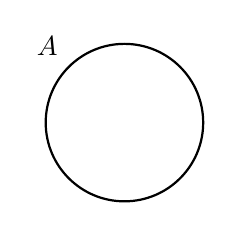
\begin{tikzpicture}[thick]
% Circle with label
\node[draw,
    circle,
    minimum size =2cm,
    label=135:$A$] (circle1) at (0,0){};
\end{tikzpicture} \]

Given two sets $A,B$ there are now four possibilities for all objects in the universe:
\begin{enumerate}
\item outside both $A$ and $B$;
\item inside $A$, but not inside $B$;
\item inside $B$, but not inside $A$;
\item inside both $A$ and $B$.
\end{enumerate}
We correspondingly divide the paper into four regions:
\[ 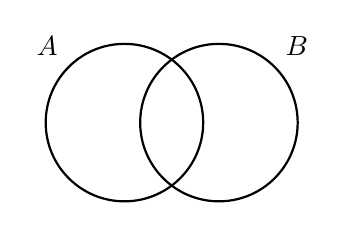
\begin{tikzpicture}[thick]
% Set A
\node [draw,
    circle,
    minimum size =2cm,
    label={135:$A$}] (A) at (0,0){};
% Set B
\node [draw,
    circle,
    minimum size =2cm,
    label={45:$B$}] (B) at (1.2,0){};
\end{tikzpicture} \]

For three sets $A,B,C$ the picture becomes:
\[ 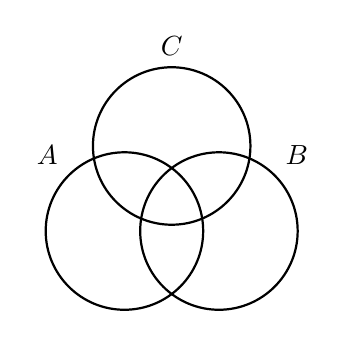
\begin{tikzpicture}[thick]
% Set A
\node[draw,circle,minimum size =2cm,label={135:$A$}] (A) at (0,0) {};

% Set B
\node[draw,circle,minimum size =2cm,label={45:$B$}] (B) at (1.2,0) {};

% Set C
\node[draw,circle,minimum size =2cm,label=$C$] (C) at (0.6,1.08) {};
\end{tikzpicture} \]

If we want to show that one set is a subset of another set, e.g\ $B\subset A$, then we can represent this as follows:
\[ 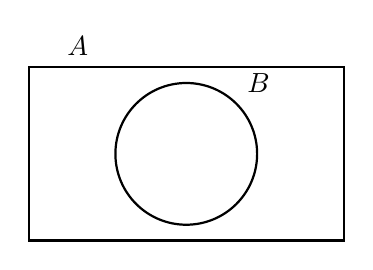
\begin{tikzpicture}[thick]
% Set A
\node [draw,
    rectangle,
    minimum width =4cm,
	minimum height = 2.2cm,
    label={135:$A$}] (A) at (0,0){};
% Set B
\node [draw,
    circle,
    minimum size =1.8cm,
    label={45:$B$}] (B) at (0,0){};
\end{tikzpicture} \]

Expressions talking about sets can be expressed by shading regions of Venn diagrams. For example $A\cup B$:
\[ 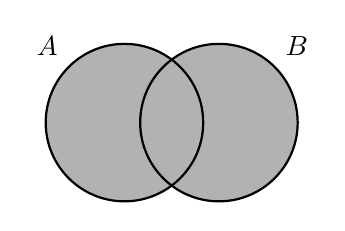
\begin{tikzpicture}[thick,
    set/.style = {circle,
        minimum size = 2cm,
        fill=black!30}]

% Set A
\node[set,label={135:$A$}] (A) at (0,0) {};

% Set B
\node[set,label={45:$B$}] (B) at (1.2,0) {};

% Circles outline
\draw (0,0) circle(1cm);
\draw (1.2,0) circle(1cm);
\end{tikzpicture} \]

\subsection{Operations on sets}
\subsubsection{Intersection}
\begin{definition}
The \udef{intersection} of an object $\mathcal{E}$ is a set $\bigcap \mathcal{E}$ defined by
\[ \bigcap \mathcal{E} \defeq \left\{ x\in \bigcup\mathcal{E} \;|\; \forall X\in \mathcal{E}: x\in X \right\}. \]
\end{definition}
As before, for the union, we define
\[ A\cap B \defeq \bigcap \{A,B\}. \]

The intersection $A\cap B$ can be represented in a Venn diagram as follows:
\[ 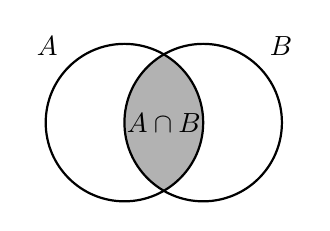
\begin{tikzpicture}[thick,
    set/.style = {circle,
        minimum size = 2cm}]

% Set A
\node[set,label={135:$A$}] (A) at (0,0) {};

% Set B
\node[set,label={45:$B$}] (B) at (1,0) {};

% Intersection
\begin{scope}
    \clip (0,0) circle(1cm);
    \clip (1,0) circle(1cm);
    \fill[black!30](0,0) circle(1cm);
\end{scope}

% Circles outline
\draw (0,0) circle(1cm);
\draw (1,0) circle(1cm);

% Set intersection label
\node at (0.5,0) {$A\cap B$};
\end{tikzpicture} \]

\begin{proposition}
Let $A, B$ be non-empty sets. Then
\begin{enumerate}
\item $A \subseteq B \implies \bigcap B\subseteq \bigcap A$;
\item $\bigcap(A\cup B) = (\bigcap A)\cup (\bigcap B)$.
\end{enumerate}
These statements hold for all sets $A,B$ iff we use an unrelativised intersection (TODO!).
\end{proposition}

\begin{definition}
Let $A,B$ be sets. We call $A$ and $B$ \udef{disjoint} if $A\cap B = \emptyset$. We write $A\perp B$.

A family of sets $\mathcal{E}$ is called \udef{pairwise disjoint} if $\forall A,B\in\mathcal{E}: A\perp B$.
\end{definition}
The notation $A\perp B$ is not standard in general set theory, but is somewhat standard for disjoint elements in lattice theory.

\begin{definition}
Let $A,B$ be sets. We call the union $A\cup B$ a \udef{(inner) disjoint union} if $A$ and $B$ are disjoint. We may write $A\uplus B$ for the union if it is disjoint.

If a family of sets $\mathcal{E}$ is pairwise disjoint, we may denote its union $\biguplus \mathcal{E}$.
\end{definition}

\begin{definition}
Let $\mathcal{A},\mathcal{B}$ be families of sets. We say $\mathcal{A}$ and $\mathcal{B}$ \udef{mesh}, denoted $\mathcal{A} \# \mathcal{B}$ if $A$ and $B$ are not disjoint, $A\cap B \neq \emptyset$, for all $A\in \mathcal{A}$ and $B\in\mathcal{B}$.

We write $A \# \mathcal{B}$ for $\{A\}\# \mathcal{B}$ and $A\# B$ for $\{A\}\#\{B\}$.
\end{definition}

\subsubsection{Difference}
\begin{definition}
Given two objects $A,B$, we define the \udef{difference} as
\[A\setminus B \defeq \setbuilder{ x\in A}{x\notin B}. \]
\end{definition}
The difference $A\setminus B$ can be represented in a Venn diagram as follows:
\[ 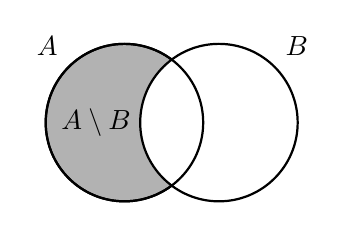
\begin{tikzpicture}[thick,
    set/.style = {circle,
        minimum size = 2cm}]

% Set A
\node[set,draw,fill=black!30,label={135:$A$}] (A) at (0,0) {};

% Set B
\node[set,draw,fill=white,label={45:$B$}] (B) at (1.2,0) {};

% Circles outline
\draw (0,0) circle(1cm);

% Set label
\node at (-0.36,0) {$A\setminus B$};
\end{tikzpicture} \]

\begin{proposition}[De Morgan's laws]
Let $A,B,C$ be sets. Then
\begin{align*}
C\setminus (A\cap B) &= (C\setminus A)\cup(C\setminus B) \\
C\setminus (A\cup B) &= (C\setminus A)\cap(C\setminus B)
\end{align*}
This can be extended to arbitrary families of sets:
\begin{align*}
C\setminus\left(\bigcup \mathcal{E}\right) &= \bigcap\setbuilder{C\setminus A}{A\in\mathcal{E}} \\
C\setminus\left(\bigcap \mathcal{E}\right) &= \bigcup\setbuilder{C\setminus A}{A\in\mathcal{E}}
\end{align*}
where $\mathcal{E}$ is a family of sets.
\end{proposition}
\begin{lemma}
Let $\mathcal{E}$ be a family of sets and $A$ a set. Then
\[ \bigcup \mathcal{E} \setminus A = \bigcup\setbuilder{X\setminus A}{X\in\mathcal{E}} \qquad\text{and}\qquad \bigcap \mathcal{E} \setminus A = \bigcap\setbuilder{X\setminus A}{X\in\mathcal{E}}. \]
\end{lemma}

\begin{lemma} \label{differenceProperties}
Let $A,B,C$ be sets. Then
\begin{enumerate}
\item $(A\setminus B)\setminus C = A\setminus (B\cup C)$;
\item $A\setminus (B\setminus C) = (A\setminus B) \cup (A\cap C)$;
\end{enumerate}
and
\begin{enumerate} \setcounter{enumi}{2}
\item $(A\setminus B)\cap C = (A\cap C)\setminus B = A\cap (C\setminus B)$;
\item $(A\setminus B)\cup C = (A\cup C)\setminus (B\setminus C)$;
\end{enumerate}
and
\begin{enumerate} \setcounter{enumi}{4}
\item $A\setminus A = \emptyset$;
\item $\emptyset\setminus A = \emptyset$;
\item $A\setminus \emptyset = A$.
\end{enumerate}
\end{lemma}

\subsubsection{Symmetric difference}
\begin{definition}
We define the \udef{symmetric difference} of two sets $A,B$ as
\[ A \symdiff B \defeq (A\setminus B)\cup(B\setminus A). \]
This is equivalent to $A\symdiff B = \setbuilder{x\in A\cup B}{(x\in A)\oplus (x\in B)}$.
\end{definition}

The symmetric difference $A\symdiff B$ can be represented in a Venn diagram as follows:
\[ 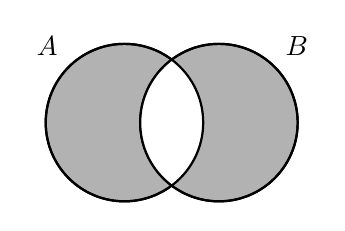
\begin{tikzpicture}[thick,
    set/.style = {circle,
        minimum size = 2cm}]

% Set A
\node[set,draw,fill=black!30,label={135:$A$}] (A) at (0,0) {};

% Set B
\node[set,draw,fill=black!30,label={45:$B$}] (B) at (1.2,0) {};

\begin{scope}
    \clip (0,0) circle(1cm);
    \clip (1.2,0) circle(1cm);
    \fill[white](0,0) circle(1cm);
\end{scope}

% Circles outline
\draw (0,0) circle(1cm);
\draw (1.2,0) circle(1cm);
\end{tikzpicture} \]

\begin{lemma}
Let $A,B,C$ be sets. Then
\begin{align*}
A\symdiff \emptyset &= A \\
A\symdiff B = \emptyset &\iff A = B
\end{align*}
and
\begin{align*}
A \symdiff B &= B \symdiff A \\
(A \symdiff B) \symdiff C &= A \symdiff (B \symdiff C) \\
A \symdiff C &= (A \symdiff B)\symdiff(B \symdiff C).
\end{align*}
\end{lemma}

\subsection{Identities and equivalences}
\subsubsection{Identities involving families of sets}
\begin{lemma}
Let $\mathcal{F}, \mathcal{G}$ be families of sets such that $\mathcal{F}\subseteq \mathcal{G}$. Then
\begin{enumerate}
\item $\bigcup \mathcal{F} \subseteq \bigcup \mathcal{G}$;
\item $\bigcap \mathcal{F} \supseteq \bigcup \mathcal{G}$.
\end{enumerate}
\end{lemma}

\subsubsection{Set operations and statements characterised}
\begin{lemma}
Let $A,B$ be sets. Then
\begin{enumerate}
\item $\begin{aligned}[t]
A\cap B &= A\setminus (A\setminus B) \\
&= B\setminus (A\symdiff B) \\
&= A\symdiff (A\setminus B);
\end{aligned}$
\item $\begin{aligned}[t]
A\cup B &= (A\symdiff B)\cup A \\
&= (A\symdiff B)\symdiff(A\cap B) \\
&= (A\setminus B)\cup B;
\end{aligned}$
\item $\begin{aligned}[t]
A\symdiff B &= (A\cup B)\setminus (A\cap B) \\
&= (A\symdiff C)\symdiff(C\symdiff B)
\end{aligned}$

for any set $C$;
\item $\begin{aligned}[t]
A\setminus B &= A\setminus (A\cap B) \\
&= A\cap(A\symdiff B) \\
&= (A\cup B)\symdiff B \\
&= A\symdiff (A\cap B);
\end{aligned}$
\end{enumerate}
\end{lemma}

\begin{lemma}
Let $A$ be a set. Then the following are equivalent:
\begin{enumerate}
\item $A$ is empty;
\item $A\cup B\subseteq B$ for every set $B$;
\item $A\subseteq B$ for every set $B$;
\item $A\subseteq (B\setminus A)$ for some set $B$;
\item $A\subseteq (B\setminus A)$ for every set $B$;
\item $\emptyset \setminus A= A$.
\end{enumerate}
\end{lemma}

\begin{lemma}
Let $A,B$ be sets. Then following are equivalent:
\begin{enumerate}
\item $A\subseteq B$;
\item $A\cap B = A$;
\item $A\cup B = B$;
\item $A\symdiff B = B\setminus A$;
\item $A\symdiff B \subseteq B\setminus A$
\item $A\setminus B = \emptyset$.
\end{enumerate}
For any universe set $\Omega$ such that $A,B\subset \Omega$ the above is also equivalent to
\begin{enumerate}\setcounter{enumi}{4}
\item $\Omega\setminus B \subseteq \Omega\setminus A$;
\item $(\Omega\cap A)\setminus B = \emptyset$;
\item $(\Omega\setminus A)\cup B = \Omega$.
\end{enumerate}
\end{lemma}
\begin{corollary}
Let $A,B$ be sets. Then following are equivalent:
\begin{enumerate}
\item $A=B$;
\item $A\symdiff B = \emptyset$;
\item $A\setminus B = B\setminus A$.
\end{enumerate}
\end{corollary}
\begin{corollary} \label{setPerpInequality}
Let $A,B\subseteq \Omega$ be sets. Then following are equivalent:
\begin{enumerate}
\item $A\perp B$;
\item $A \subseteq \Omega\setminus B$;
\item $B \subseteq \Omega\setminus A$.
\end{enumerate}
\end{corollary}

\subsubsection{Distributivity}
TODO: tables complete / correct?? TODO: only works for relativised intersection.
\begin{lemma}
We say $*$ left distributes over $\bullet$ if
\[ A*(B\bullet C) = (A*B)\bullet (A*C) \qquad\text{for all sets $A,B,C$.} \]
This gives the table
\[ \begin{array}{c | c c c c c}
\text{\diagbox{$*$}{$\bullet$}} & \cup & \cap & \symdiff & \setminus & \times \\ \hline
\cup & \checkmark & \checkmark &  & & \\
\cap & \checkmark & \checkmark & \checkmark & \checkmark & \\
\symdiff &  &  &  & & \\
\setminus &  &  &  & & \\
\times & \checkmark & \checkmark &  & \checkmark &
\end{array} \]
\end{lemma}

\begin{lemma}
We say $*$ right distributes over $\bullet$ if
\[ (A\bullet B)*C = (A*C)\bullet (B*C) \qquad\text{for all sets $A,B,C$.} \]
This gives the table
\[ \begin{array}{c | c c c c c}
\text{\diagbox{$*$}{$\bullet$}} & \cup & \cap & \symdiff & \setminus & \times \\ \hline
\cup & \checkmark & \checkmark &  & & \\
\cap & \checkmark & \checkmark & \checkmark & \checkmark & \\
\symdiff &  &  &  & & \\
\setminus & \checkmark & \checkmark & \checkmark & \checkmark & \\
\times & \checkmark & \checkmark &  & \checkmark &
\end{array} \]
\end{lemma}

TODO: intersection distributes over disjoint union.

\begin{lemma} \label{unionIntersectionLabelSet}
Let $\mathcal{I}$ be a family of index sets and let $A_i$ be a set for all $i\in \bigcup \mathcal{I}$. Then
\begin{enumerate}
\item $\bigcup_{i\in \bigcup \mathcal{I}} A_i = \bigcup_{I\in \mathcal{I}}\bigcup_{i\in I} A_i$;
\item $\bigcap_{i\in \bigcap \mathcal{I}} A_i = \bigcap_{I\in \mathcal{I}}\bigcap_{i\in I} A_i$;
\item $\bigcup_{i\in \bigcap \mathcal{I}} A_i \subseteq \bigcap_{I\in \mathcal{I}}\bigcup_{i\in I} A_i$;
\item $\bigcap_{i\in \bigcup \mathcal{I}} A_i \supseteq \bigcup_{I\in \mathcal{I}}\bigcap_{i\in I} A_i$.
\end{enumerate}
\end{lemma}
\begin{proof}
(1) We calculate
\begin{align*}
x\in \bigcup_{i\in \bigcup \mathcal{I}} A_i &\iff \exists i\in \bigcup \mathcal{I}: x\in A_i \\
&\iff \exists i: (i\in \bigcup \mathcal{I}) \land (x\in A_i) \\
&\iff \exists i: (\exists I \in \mathcal{I}: i\in I) \land (x\in A_i) \\
&\iff \exists i: \exists I: (I \in \mathcal{I}) \land (i\in I) \land (x\in A_i) \\
&\iff \exists I\in \mathcal{I}: \exists i \in I: x\in A_i \\
&\iff x\in \bigcup_{I\in \mathcal{I}}\bigcup_{i\in I} A_i
\end{align*}

(2) Replace $\exists$ by $\forall$ and $\land$ by $\Rightarrow$ in the proof of (1).

(3) We calculate
\begin{align*}
x\in \bigcup_{i\in \bigcap \mathcal{I}} A_i &\iff \exists i\in \bigcap \mathcal{I}: x\in A_i \\
&\iff \exists i: (i\in \bigcap \mathcal{I}) \land (x\in A_i) \\
&\iff \exists i: (\forall I \in \mathcal{I}: i\in I) \land (x\in A_i) \\
&\iff \exists i: (\forall I: (I \in \mathcal{I}) \Rightarrow (i\in I)) \land (x\in A_i) \\
&\implies \exists i: \forall I: (I \in \mathcal{I}) \Rightarrow ((i\in I) \land (x\in A_i)) \\
&\implies \forall I: \exists i: (I \in \mathcal{I}) \Rightarrow ((i\in I) \land (x\in A_i)) \\
&\iff \forall I: (I \in \mathcal{I}) \Rightarrow (\exists i:(i\in I) \land (x\in A_i)) \\
&\iff \forall I\in \mathcal{I}: \exists i \in I: x\in A_i \\
&\iff x\in \bigcap_{I\in \mathcal{I}}\bigcup_{i\in I} A_i
\end{align*}

(4) TODO
\end{proof}

For more identities, see \url{https://en.wikipedia.org/wiki/List_of_set_identities_and_relations}.


\chapter{Relations and functions}
\section{Pairs}
\begin{definition}
A definition of $(a,b)$ for all $a,b$ is called an \udef{(ordered) pair operation} if it satisfies
\begin{itemize}
\item $(a,b) = (x,y) \iff (a=x)\land (b=y)$;
\item for all sets $A,B$, $\setbuilder{(a,b)}{a\in A\land b\in B}$ is a set.
\end{itemize}
We call $\setbuilder{(a,b)}{a\in A\land b\in B}$ the \udef{Cartesian product} of $A$ and $B$ and denote it $A\times B$.
\end{definition}
Note that for the second condition it is enough to check that $A\times B$ is a subset of some set $S$. Then, by separation, $A\times B$ is the set
\[ A\times B = \setbuilder{x\in S}{\exists a\in A:\exists b\in B: x = (a,b)}. \]

\begin{lemma}
Let $A$ be a set. Then
\[ A\times \emptyset = \emptyset = \emptyset\times A. \]
\end{lemma}

\begin{lemma} \label{productUnionIntersection}
Let $A,B,C$ be sets. Then
\begin{enumerate}
\item $(A\cup B)\times C = A\times C \cup B\times C$;
\item $(A\uplus B)\times C = A\times C \uplus B\times C$;
\item $(A\cap B)\times C = A\times C\cap B\times C$.
\end{enumerate}
\end{lemma}

\begin{definition}
Let $p = (a,b)$ be a pair, we use $\pi_1(p)$ to denote the first element of $p$ and $\pi_2(p)$ to denote the second element:
\[ (a,b) = p = (\pi_1(p),\pi_2(p)). \]
We can convert a pair to a set:
\[ \operatorname{set}((a,b)) = \{a,b\}. \]
\end{definition}
\subsection{Defining pairs}
\subsubsection{The Kuratowski pair}
\begin{definition}
The \udef{Kuratowski pair} is defined as
\[ (a,b) \defeq \{\{a\}, \{a,b\}\} \]
\end{definition}
Note that when $a=b$ we have
\[ (a,a) = \{\{a\},\{a,a\}\} = \{\{a\},\{a\}\} = \{\{a\}\}. \]
\begin{lemma}
Given a Kuratowski pair $p = (a,b)$, we can extract the first element $\pi_1(p)$ and the second element $\pi_2(p)$ as follows:
\begin{align*}
\pi_1(p) &= \bigcup\bigcap p; \\
\pi_2(p) &= \bigcup\left\{ x\in\bigcup p\;|\; \left[\bigcup p \neq \bigcap p\right] \implies \left[ x\notin \bigcap p \right] \right\}.
\end{align*}
The Kuratowski pair can be converted to a set by
\[ \operatorname{set}(p) = \bigcup p. \]
\end{lemma}
The construction ``$\left[\bigcup p \neq \bigcap p\right] \implies$'' in the formula for $\pi_2(p)$ is there so that it still works in case the first and second elements are the same.
\begin{proposition}
The Kuratowski pair is adequate, in that is satisfies
\[ (a,b) = (x,y) \iff (a=x)\land (b=y) \]
and the Cartesian product is a set.
\end{proposition}
\begin{proof}
If $(a=x)\land (b=y)$, then
\[ \{\{a\},\{a,b\}\} = \{\{x\},\{x,y\}\} \]
and thus $(a,b) = (x,y)$.

Now assume $(a,b) = (x,y)$. We consider two cases: $a=b$ and $a\neq b$.
\begin{itemize}[leftmargin=2cm]
\item[$\boxed{a=b}$] Then $(a,b) = \{\{a\},\{a,a\}\} = \{\{a\}\} = (x,y)$ and thus $\{x\} = \{x,y\} = \{a\}$ by extensionality. This implies $a=x=y$ and thus $(a=x)\land (b=y)$.
\item[$\boxed{a\neq b}$] Now $(a,b) = (x,y)$ implies
\[ \{\{a\},\{a,b\}\} = \{\{x\},\{x,y\}\}. \]
By extensionality, either $\{x\} = \{a\}$ or $\{x\} = \{a,b\}$. In the second option $a=x=b$ and thus $a=b$ which is a contradiction. So $x=a$.

Again by extensionality, either $\{x,y\} = \{a\}$ or $\{x,y\} = \{a,b\}$. In the first case $(x,y)$ would be a singleton and then by equality so would $(a,b)$, yielding a contradiction. Thus $\{x,y\} = \{a,b\}$. We know $a=x$ and $b\neq a$, so by extensionality $b=y$.
\end{itemize}
To prove the Cartesian product $A\times B$ is a set, notice that
\begin{align*}
a\in A, b\in B &\implies \{a\},\{a,b\}\subseteq A\cup B \implies \{a\},\{a,b\}\in \powerset(A\cup B)\\
&\implies \{\{a\},\{a,b\}\}\subseteq \powerset(A\cup B) \implies \{\{a\},\{a,b\}\}\in \powerset(\powerset(A\cup B)) \\
&\implies (a,b) \in \powerset(\powerset(A\cup B)).
\end{align*}
and $\powerset(\powerset(A\cup B))$ is a set. So
\[ A\times B = \{ x\in \powerset(\powerset(A\cup B))\;|\; \exists a\in A:\exists b\in B: x = (a,b) \} \]
is a set.
\end{proof}
\subsubsection{The short variant}
We can also define a pair as
\[ (a,b) \defeq \{a,\{a,b\}\} \]
The advantage of this short definition is fewer braces. Some disadvantages include:
\begin{enumerate}
\item If $a$ and $b$ have the same type, $a$ and $\{a,b\}$ do not have the same type.
\item In order to prove adequacy, we need a new axiom, the axiom of regularity.
\end{enumerate}
\subsubsection{Using $0,1$}
Suppose we have decided on two special, distinct objects $0,1$. Then we can define
\[ (a,b) \defeq \{\{0,a\},\{1,b\}\}. \]
\begin{proposition}
This definition satisfies the requirements for a pair.
\end{proposition}
\begin{proof}
Assuming $(a=x)\land (b=y)$, it is clear that $(a,b)=(x,y)$ as sets by extensionality.

Now assume $(a,b)=(x,y)$. In this implementation a pair always has two elements as a set. The reasoning by extensionality is simple and only slightly more difficult if $a,b,x,y$ are equal to $0$ or $1$.

The Cartesian product is a subset of $\powerset(\powerset(A\cup B\cup \{0,1\}))$ and thus a set.
\end{proof}
\subsubsection{Wiener pair}
The Wiener definition of a pair is
\[ (a,b) \defeq \{\{\emptyset,\{a\}\},\{\{b\}\}\}. \]
\begin{proposition}
This definition satisfies the requirements for a pair.
\end{proposition}

\subsection{Structured sets}
\begin{definition}
A \udef{structured set} is a pair $U = (A,S)$ where $A$ is a set and $S$ is an arbitrary object.
\begin{itemize}
\item $A$ is the \udef{field} or \udef{space} of $U$, written $\operatorname{Field}(U)$;
\item $S$ is the \udef{frame} of $U$.
\end{itemize}
If we write $x\in U$, we mean $x\in \operatorname{Field}(U)$.
\end{definition}

Often the frame $S$ is a $n$-tuple. In this case we may write the structured set as an $n+1$-tuple by concatenating the field and the frame. e.g\ $(A,(S_1,S_2,S_3))$ becomes $(A,S_1,S_2,S_3)$.

\section{Relations}
\begin{definition}
Let $A,B$ be sets and $G$ any subset of the Cartesian product $A\times B$. A \udef{(binary) relation} $R$ on $(A, B)$ is a tuple $(G,(A,B))$. The \udef{graph} of the binary relation $R$ is the set $\graph(R) \defeq G$.

We write
\[ xRy \defequiv  (x,y)\in \graph(R) \]
and say $x$ is \udef{left related} to $y$ or $y$ is \udef{right related} to $x$.

We call
\begin{itemize}
\item $\dom(R) \defeq A$ the \udef{domain} of the relation;
\item $\codom(R) \defeq B$ the \udef{codomain} of the relation.
\end{itemize}
A relation $R$ is \udef{homogeneous} or an \udef{endorelation} if $\dom(R) = \codom(R)$.
If we say $R$ is a (homogenous) relation on $A$, we mean $\dom(R) = A = \codom(R)$. 

A relation is \udef{heterogeneous} is the domain and codomain are different.
\end{definition}

Often we will write $R \subseteq S$ as a shorthand for $\graph(R)\subseteq \graph(S)$. Similarly we may write $R\cup S$, $R\cap S$ etc.



\begin{definition}
Let $A,B$ be sets. We have the following relations:
\begin{itemize}
\item the \udef{empty relation} $E_{A,B}$ on $(A, B)$ has graph $\emptyset$;
\item the \udef{universal relation} $U_{A,B}$ on $(A, B)$ has graph $A\times B$;
\item the \udef{identity relation} $\id_A$ on $A$ has graph $\setbuilder{(x,y)\in A\times A}{x=y}$.
\end{itemize}
We may also write $U_A$ instead of $U_{A,A}$ and $E_A$ instead of $E_{A,A}$.
\end{definition}
The identity relation on $A$ is also known as the \udef{diagonal relation} on $A$.

\begin{lemma}
Let $A,B,C,D$ be sets. Then
\begin{enumerate}
\item $\id_{A\cup B} = \id_A\cup \id_B$ and $\id_{A\cap B} = \id_A\cap \id_B$;
\item $E_{A\cup C, B\cup D} = E_{A,B}\cup E_{C,D}$ and $E_{A\cap C, B\cap D} = E_{A,B}\cap E_{C,D}$;
\item $U_{A\cap C, B\cap D} = U_{A,B}\cap U_{C,D}$.
\end{enumerate}
\end{lemma}
Note that the equalities mean the graphs are equal. The relations are not the same as they have different domains and codomains.
\begin{proof}
(1) Assume $(x,x)\in \id_{A\cup B}$. We have the equivalences
\[ (x\in A)\lor (x\in B) \iff \Big((x,x)\in \id_A\Big) \lor \Big((x,x)\in\id_B\Big) \iff (x,x)\in \id_A\cup \id_B. \]
For the second part replace $\lor$ with $\land$.

(2) Trivial because all sets are $\emptyset$.

(3) Take $(x,y)\in U_{A\cap C, B\cap D}$. We have the equivalences
\begin{align*}
(x\in A\cap C) \land (y\in B\cap D) &\iff (x\in A)\land (y\in B)\land(x\in C)\land(y\in D) \\
&\iff \big((x,y)\in U_{A, B})\big)\land\big((x,y)\in U_{A, B}\big) \\
&\iff (x,y)\in U_{A,B}\cap U_{C,D}.
\end{align*}
\end{proof}


\begin{definition}
Let $R$ be a binary relation. We say
\begin{itemize}
\item $x$ is \udef{related to} or \udef{comparable with} $y$ if $xRy$ or $yRx$; we denote this $x\nparallel_R y$ or just $x\nparallel y$;
\item $x$ is \udef{unrelated to}, \udef{incomparable with} or \udef{parallel with} $y$ if neither $xRy$ nor $yRx$; we denote this $x\parallel_R y$ or just $x\parallel y$.
\end{itemize}
\end{definition}

\subsection{Relations and sets}
\subsubsection{Images and preimages}
\begin{definition}
Let $R$ be a relation on $(A, B)$.
\begin{itemize}
\item The \udef{image} of a subset $X\subset A$ under $R$ is the set
\[ X_R \defeq \setbuilder{b\in B}{\exists x\in X: xRb}. \]
\item The \udef{preimage} of a subset $Y\subset B$ under $R$ is the set
\[ _RY \defeq \setbuilder{a\in A}{\exists y\in Y: aRy}. \]
\end{itemize}
In particular for $X=A$ and $Y=B$:
\begin{enumerate}
\item The set $A_R$ is the \udef{active codomain}, \udef{codomain of definition}, \udef{image} or \udef{range} of the relation, also denoted $\im(R)$.
\item The set $_RB$ is the \udef{active domain}, \udef{domain of definition}, \udef{preimage} or \udef{prerange} of the relation, also denoted $\preim(R)$.
\end{enumerate}
In particular for $X = \{x\}$ and $Y = \{y\}$ we define:
\begin{itemize}
\item $xR \defeq \{x\}_R$;
\item $Ry \defeq {_R\{x\}}$.
\end{itemize}
We call such images and preimages \udef{principle} images and preimages.
\end{definition}

A relation is completely characterised by its principal images.
\begin{lemma} \label{relationFromPrincipalImages}
Let $R$ be a relation on $(A, B)$, $x\in A$ and $y\in B$. Then
\[ x\in Ry \iff xRy \iff xR \ni y. \]
\end{lemma}
Principal images atoms in lattice of images??

\begin{lemma}
Let $R$ be a relation on $(A, B)$, $X\subset A$ and $Y\subset B$. Then
\begin{enumerate}
\item $X_R = {_{R^\transp}X}$;
\item $_RX = X_{R^\transp}$.
\end{enumerate}
In particular $xR = R^\transp x$ and $Ry = yR^\transp$ for all $x\in A$ and $y\in B$.
\end{lemma}

TODO: atomicity / atomistic ??
\begin{lemma}
Let $R$ be a relation on $(A, B)$, $X\subset A$ and $Y\subset B$. Then
\begin{enumerate}
\item $X_R = \displaystyle\bigcup_{x\in X}xR = \bigcup \setbuilder{xR}{x\in X}$;
\item $_RY = \displaystyle\bigcup_{y\in Y}Ry = \bigcup \setbuilder{Ry}{y\in Y}$.
\end{enumerate}
\end{lemma}


\begin{corollary} \label{monotonicityImage}
Let $R$ be a relation on $(A, B)$ and $X,Y\subset A$. Then
\begin{enumerate}
\item if $X\subseteq Y$, then $X_R \subseteq Y_R$;
\item if $X\subseteq Y$, then ${_RX} \subseteq {_RY}$.
\end{enumerate}
\end{corollary}
\begin{proof}
(1) We can write $Y = X \cup (Y\setminus X)$. Then
\[ Y_R = \bigcup \setbuilder{xR}{x\in Y} = \bigcup \setbuilder{xR}{x\in X}\cup\setbuilder{xR}{x\in (Y\setminus X)} = X_R \cup (Y\setminus X)_R \supseteq X_R. \]

(2) Similar.
\end{proof}
\begin{corollary} \label{imageRelation} \label{preimageRelation}
Let $R$ be a relation on $(A, B)$, $X,Y\subset A$ and $Z,W\subset B$. Then
\begin{enumerate}
\item $(X\cup Y)_R = X_R\cup Y_R$;
\item $(X\cap Y)_R \subseteq X_R\cap Y_R$;
\item $(X\setminus Y)_R \supseteq X_R\setminus Y_R$;
\item $(X\symdiff Y)_R \supseteq X_R\symdiff Y_R$.
\end{enumerate}
and
\begin{enumerate}
\item $_R(Z\cup W) = {_RZ}\cup {_RW}$;
\item $_R(Z\cap W) \subseteq {_RZ}\cap {_RW}$;
\item $_R(Z\setminus W) \supseteq {_RZ}\setminus {_RW}$;
\item $_R(Z\symdiff W) \supseteq {_RZ}\symdiff {_RW}$.
\end{enumerate}
\end{corollary}
\begin{proof}\mbox{}

(1) $\begin{aligned}[t]
(X\cup Y)_R &= \bigcup \setbuilder{xR}{x\in (X\cup Y)} = \bigcup \setbuilder{xR}{x\in X}\cup \setbuilder{xR}{x\in Y} \\
&= \left(\bigcup \setbuilder{xR}{x\in X}\right)\cup \left(\bigcup \setbuilder{xR}{x\in Y}\right) = X_R \cup Y_R.
\end{aligned}$

(2) We have both $X\cap Y \subseteq X$ and $X\cap Y \subseteq Y$, so $(X\cap Y)_R \subseteq X_R$ and $(X\cap Y)_R \subseteq Y_R$ by \ref{monotonicityImage}. Thus $(X\cap Y)_R \subseteq X_R\cap Y_R$.

TODO: use lattice properties

(3), (4) TODO
\end{proof}


\subsubsection{Left and right bounds}
\begin{definition}
Let $R$ be a relation on $(A, B)$, $X\subseteq A$ and $Y\subseteq B$.
\begin{itemize}
\item A \udef{right bound} (or \udef{upper bound}) of $X$ under $R$ is an element $b\in B$ such that $b$ is right related to all $x\in X$. We denote the set of right bounds by
\[ X^R \defeq \setbuilder{b\in B}{\forall x\in X: xRb}. \]
\item A \udef{left bound} (or \udef{lower bound}) of $Y$ under $R$ is an element $a\in A$ such that $a$ is left related to all $y\in Y$. We denote the set of left bounds by
\[ ^RY \defeq \setbuilder{a\in A}{\forall y\in Y: aRy}. \]
\end{itemize}
The sets $X^R$ and $^RY$ are also called \udef{polars}.\footnote{Birkhoff states (TODO ref) that the term ``polar'' was chosen due to the link with the polars of conic sections.}

In particular for $X=A$ and $Y=B$:
\begin{enumerate}
\item The set $A^R$ is referred to as the \udef{top} of $\sSet{R,(A,B)}$.
\item The set $^RB$ is the \udef{bottom} of $\sSet{R,(A,B)}$.
\end{enumerate}
\end{definition}
Note that the definitions of the polars is similar to the definition of the image/preimage. The only difference is that ``$\exists$'' is replaced by ``$\forall$''.

Consequently, we can state results similar to the ones above.

\begin{lemma}
Let $R$ be a relation on $(A, B)$, $X\subset A$ and $Y\subset B$. Then
\begin{enumerate}
\item $X^R = {^{R^\transp}X}$;
\item $^RX = X^{R^\transp}$.
\end{enumerate}
\end{lemma}

\begin{lemma} \label{boundsFromPrincipalImages}
Let $R$ be a relation on $(A, B)$, $X\subset A$ and $Y\subset B$. Then
\begin{enumerate}
\item $X^R = \displaystyle\bigcap_{x\in X}xR = \bigcap \setbuilder{xR}{x\in X}$;
\item $^RY = \displaystyle\bigcap_{y\in Y}Ry = \bigcap \setbuilder{Ry}{y\in Y}$.
\end{enumerate}
In particular for $x\in A$ and $y\in B$:
\begin{enumerate}
\item $\{x\}^R = xR = \{x\}_R$;
\item $^R\{y\} = Ry = {_R\{y\}}$.
\end{enumerate}
\end{lemma}
TODO this only works for empty sets if we relativise the intersection!

\begin{lemma} \label{polarsCartesianProduct}
Let $R$ be a relation on $(A,B)$ and $X\subseteq A, Y\subseteq B$. Then
\[ Y\subseteq X^R \iff X\times Y \subseteq R. \]
\end{lemma}

\begin{corollary} \label{monotonicityPolars}
Let $R$ be a relation on $(A, B)$ and $X,Y\subset A$. Then
\begin{enumerate}
\item if $X\subseteq Y$, then $X^R \supseteq Y^R$;
\item if $X\subseteq Y$, then ${^RX} \supseteq {^RY}$.
\end{enumerate}
\end{corollary}
\begin{proof}
(1) We can write $Y = X \cup (Y\setminus X)$. Then
\[ Y^R = \bigcap \setbuilder{xR}{x\in Y} = \bigcap \setbuilder{xR}{x\in X}\cap\setbuilder{xR}{x\in (Y\setminus X)} = X^R \cap (Y\setminus X)^R \subseteq X^R. \]

(2) Similar.
\end{proof}
\begin{corollary} \label{polarasRelation}
Let $R$ be a relation on $(A, B)$, $X,Y\subset A$ and $Z,W\subset B$. Then
\begin{enumerate}
\item $(X\cup Y)^R \subseteq X^R\cap Y^R$;
\item $(X\cap Y)^R \supseteq X^R\cup Y^R$;
\item $(X\setminus Y)^R ? X^R\setminus Y^R$;
\item $(X\symdiff Y)^R ? X^R\symdiff Y^R$.
\end{enumerate}
and
\begin{enumerate}
\item $^R(Z\cup W) \subseteq {^RZ}\cup {^RW}$;
\item $^R(Z\cap W) \supseteq {^RZ}\cap {^RW}$;
\item $^R(Z\setminus W) ? {^RZ}\setminus {^RW}$;
\item $^R(Z\symdiff W) ? {^RZ}\symdiff {^RW}$.
\end{enumerate}
\end{corollary}
\begin{proof}\mbox{}
(1) We have both $X\cup Y \supseteq X$ and $X\cup Y \supseteq Y$, so $(X\cup Y)^R \subseteq X^R$ and $(X\cup Y)^R \subseteq Y^R$ by \ref{monotonicityImage}. Thus $(X\cup Y)^R \subseteq X^R\cap Y^R$.

(2) TODO ref order reversing function on lattice.

(3), (4) TODO
\end{proof}

\subsubsection{Extending the relation to powersets}
\begin{definition}
Let $R$ be a relation on $(A,B)$. Let $X\subseteq A$ and $Y\subseteq B$ be sets. Then we write $XRY$ if
\[ \forall x\in X \forall y\in Y: \; xRy. \]
\end{definition}

\begin{lemma}
Let $R$ be a relation on $(A,B)$. Let $X\subseteq A$ and $Y\subseteq B$ be sets. Then
\[ XRY \quad\iff\quad X \subseteq {^RY} \quad\iff\quad Y \subseteq X^R. \]
\end{lemma}

\begin{definition}
Let $R$ be a relation on $(A,B)$. Let $\mathcal{E}\subseteq \powerset(A)$. Then we define
\begin{itemize}
    \item $\mathcal{E}_R \defeq \setbuilder{X_R}{X\in \mathcal{E}}$;
    \item $\mathcal{E}^R \defeq \setbuilder{X^R}{X\in \mathcal{E}}$.
\end{itemize}
\end{definition}

\subsubsection{Greatest and least elements}
\begin{definition}
Let $\sSet{A, R}$ be a relational structure and $X\subseteq A$ a subset.
\begin{itemize}
\item A \udef{greatest element}, \udef{largest element} or \udef{maximum} of $X$ is an upper bound of $X$ that is an element of $X$. We denote the set of maxima by $\max(X) \defeq X^R\cap X$.
\item A \udef{least element}, \udef{smallest element} or \udef{minimum} of $X$ is a lower bound of $X$ that is an element of $X$. We denote the set of minima by $\min(X) \defeq {^RX}\cap X$.
\end{itemize}
We also call
\begin{itemize}
\item an element of $\sup(S) \defeq \min(X^R) = X^R \cap (X^R)^{R^\transp}$ a \udef{least upper bound}, \udef{supremum}, or \udef{join};
\item an element of $\inf(S) \defeq \max({^RX}) = X^{R^\transp} \cap (X^{R^\transp})^R$ a \udef{greatest lower bound}, \udef{infimum}, or \udef{meet}.
\end{itemize}
\end{definition}

\begin{lemma} \label{minMaxSingletons}
If $\sSet{A, R}$ is an anti-symmetric relational structure and $X\subseteq A$, then $\max(X), \min(X), \sup(X)$ and $\inf(X)$ are either singletons or empty.
\end{lemma}
\begin{proof}
We prove for $\max(X)$. The other cases follow dually or a fortiori. Let $x,y\in \max(X)$. Then $xRy$ and $yRx$, so $x=y$ by anti-symmetry.
\end{proof}
For posets we sometimes use $\max/\min/\sup/\inf$ to denote the contents of the singleton rather than the singleton itself. If the set is empty, we say the $\max/\min/\sup/\inf$ does not exist.

\begin{lemma} \label{greatestLeastElementsSubsetPoset}
Let $\sSet{P, \precsim}$ be a poset and $R\subseteq S\subseteq P$.
\begin{enumerate}
\item If $\max(R)$ and $\max(S)$ exists, then $\max(R) \precsim \max(S)$.
\item If $\min(R)$ and $\min(S)$ exists, then $\min(R) \succsim \min(S)$.
\end{enumerate}
\end{lemma}
\begin{proof}
By definition $\max(S) \succsim x$ for all $x \in S$. Now $\max(R)\in R\subseteq S$, so in particular $\max(R) \precsim \max(S)$.
\end{proof}

\begin{lemma} \label{maxSupMinInf}
If $\sSet{P, \Yleft}$ is an ordered set and $S\subseteq P$, then
\begin{enumerate}
\item $\max(S)\subset \sup(S)$;
\item $\min(S)\subset \inf(S)$.
\end{enumerate}
\end{lemma}
\begin{proof}
For (1) we calculate $\max(S) = S \cap S^u \subseteq (S^u)^l \cap S^u = \sup(S)$; (2) is dual.

TODO: post Galois??
\end{proof}

\subsubsection{Maxima and minima}
\begin{definition}
$X^{R\cup \overline{R}^\transp}\cap X$ (if anti-asymmetric = $X^{\overline{R}^\transp}\cap X$).

A \udef{maximal element} of $S$ is an element $x\in S$ such that no element $y$ is strictly greater than $x$
\end{definition}

\subsection{Converse relation}
\begin{definition}
Let $R$ be a relation on $(A, B)$. The \udef{converse} $R^\transp$ of $R$ is the relation on $B\times A$ with graph
\[ \graph(R^{\transp}) = \setbuilder{(y,x)}{(x,y)\in \graph(R)} \subset B\times A. \]
It is also known as the \udef{inverse}, \udef{transpose}, \udef{reciprocal}, \udef{opposite} or \udef{dual} of $R$.
\end{definition}

\begin{lemma}
Let $R,S$ be relations on $(A, B)$, $X\subseteq A$ and $Y\subseteq B$. Then
\begin{enumerate}
\item $(R^\transp)^\transp = R$;
\item $(R \cup S)^\transp = R^\transp \cup S^\transp$;
\item $(R \cap S)^\transp = R^\transp \cap S^\transp$;
\item $\dom(R^\transp) = \codom(R)$ and $\codom(R^\transp) = \dom(R)$;
\item $_{R^\transp}X = X_R$ and $Y_{R^\transp} = {_RY}$;
\item $\im(R^\transp) = \preim(R)$;
\item if $R\subseteq S$, then $R^\transp \subseteq S^\transp$.
\end{enumerate}
\end{lemma}

\begin{lemma}
Let $A,B$ be sets. Then
\begin{enumerate}
\item $U_{A,B}^\transp = U_{B,A}$;
\item $E_{A,B}^\transp = E_{B,A}$;
\item $\id_A^\transp = \id_A$.
\end{enumerate}
\end{lemma}

\subsection{Complementary relation}
\begin{definition}
Let $R$ be a binary relation on $(A, B)$. The \udef{complementary relation} $\overline{R}$ of $R$ is the relation on $(A, B)$ with graph
\[ \graph(\overline{R}) = \setbuilder{(x,y)}{\neg xRy}. \]
\end{definition}
\begin{lemma} \label{relationalComplementProperties}
Let $R,S$ be binary relations.
\begin{enumerate}
\item $\overline{\overline{R}} = R$;
\item $\overline{R^\transp} = \overline{R}^\transp$;
\item $\overline{R\cup S} = \overline{R}\cap \overline{S}$;
\item $\overline{R\cap S} = \overline{R}\cup \overline{S}$;
\item $U = R \cup \overline{R}$;
\item if $R \subseteq S$, then $\overline{R} \supseteq \overline{S}$.
\end{enumerate}
\end{lemma}


\begin{lemma}
Let $R$ be a relation on $(A,B)$, $x\in A$ and $y\in B$. Then
\begin{enumerate}
\item $x\overline{R} = B\setminus (xR)$;
\item $\overline{R}y = A\setminus (Ry)$.
\end{enumerate}
If $X\subseteq A$ and $Y\subseteq B$. Then
\begin{enumerate} \setcounter{enumi}{2}
\item $X_{\overline{R}} = B\setminus X^R$;
\item $_{\overline{R}}Y = A\setminus {^RY}$.
\end{enumerate}
\end{lemma}
\begin{proof}
(1) We calculate
\[ y \in x\overline{R} \iff \neg xRy \iff \neg (y\in xR) \iff y\in B\setminus (xR). \]

(2) Similar.

(3) We calculate, using (1),
\[ X_{\overline{R}} = \bigcup_{x\in X}x\overline{R} = \bigcup_{x\in X}B\setminus (xR) = B\setminus \left(\bigcap_{x\in X}xR\right) = B\setminus X^R. \]

(4) Similar.
\end{proof}
\begin{corollary}
Let $X\subseteq A$ be sets. Then
\[ X^c = X^{\overline{\id_A}}, \]
where the converse is taken with respect to $A$.
\end{corollary}
\begin{proof}
We have $X = X_{\id_A} = (X^{\overline{\id_A}})^c$.
\end{proof}

\subsection{Composition of relations}
\begin{definition}
Let $R$ be a relation on $(A, B)$ and $S$ a relation on $(B, C)$. Then the \udef{composition} of $R$ and $S$ is a new relation $R;S$ on $(A, C)$ with graph
\[ \graph(R;S) = \setbuilder{(x,z)\in A\times C}{\exists y\in B: xRy \land ySz}. \]
If $R$ and $S$ are relations such that the codomain of one is the domain of the other, they are called \udef{composable}.

If $R$ and $S$ are composable we also define the notation
\[ S\circ R \defeq R;S. \]
\end{definition}
\begin{lemma} \label{relationalComposition}
Let $R,S,T$ be composable relations.
\begin{enumerate}
\item The composition is associative: $R;(S;T) = (R;S);T$.
\item $(R;S)^\transp = S^\transp ; R^\transp$;
\item $(R\cup S);T = (R;T) \cup (S;T)$;
\item $(R\cap S);T \subseteq R;T \cap S;T$.
\end{enumerate}
\end{lemma}
\begin{proof}
TODO
\end{proof}
TODO: equality for $\cap$ with functions!!

\begin{lemma} \label{setOfRelationComposition}
Let $R,S$ be composable relations. Then for all $x,y$
\begin{enumerate}
\item $x(R;S)y \iff xR \mesh Sy$;
\item $x(\overline{R;S})y \begin{aligned}[t]
&\iff xR\perp Sy \\
&\iff xR \subseteq \overline{S}y;
\end{aligned}$
\item $x(\overline{R;\overline{S}})y \iff xR \subseteq Sy$.
\end{enumerate}
\end{lemma}
\begin{proof}
TODO
\end{proof}
\begin{corollary}
Let $R,S$ be composable relations. If $R$ is right unique, then $\overline{R;\overline{S}} = R;S$.
\end{corollary}


\begin{lemma}
Let $A,B,C,D$ be relations such that $A \subseteq B$ and $C\subseteq D$ and both $A,B$ and $C,D$ are composable, then $A;C\subseteq B;D$.
\end{lemma}
\begin{proof}
Assume the hypotheses of the lemma and let $(x,y) \in \graph(A;C)$. Then there exists a $z$ such that $xAz$ and $zCy$. By hypothesis this means $xBz$ and $zDy$, so $x(B;D)y$.
\end{proof}

\begin{lemma} \label{universalQuantificationForCompositionSuperset}
Let $R,S$ be composable and $T$ a relation. Then
\[ R;S \subseteq T \qquad\iff\qquad \forall x,y,z:\; xRy \land ySz \implies xTz. \]
\end{lemma}

\begin{lemma} \label{compositionCanonicalRelations}
Let $A,B,X, Y$ be sets and $R$ a relation on $(A, B)$. Then
\begin{enumerate}
\item $\id_A;R = R = R;\id_B$;
\item if $S,T\subseteq A$, then $\id_{S};\id_{T} = \id_{S\cap T}$;
\item $E_{X,A};R = E_{X,B}$ and $R; E_{B,Y} = E_{A,Y}$;
\item $U_{X,A};R = \U_{X,A_R}$ and $R; U_{B,Y} = U_{_RB, Y}$;
\item $U_{X,A};R;U_{B,Y} = \begin{cases}
U_{X,Y} & \graph(R) \neq \emptyset \\
E_{X,Y} & \graph(R) = \emptyset.
\end{cases}$
\end{enumerate}
\end{lemma}

\begin{lemma} \label{kernelInclusions}
Let $R$ be a relation. Then
\begin{enumerate}
\item $\id_{\preim(R)} \subseteq R;R^\transp \subseteq U_{\preim(R)}$;
\item $\id_{\im(R)} \subseteq R^\transp;R \subseteq U_{\im(R)}$.
\end{enumerate}
\end{lemma}
\begin{corollary}
Let $R$ be a relation on $(A,B)$, then
\begin{enumerate}
\item $R \subseteq R;R^\transp;R$;
\item $(\id_A \cap R;R^\transp);R = R = R;(\id_{B}\cap R^\transp;R)$.
\end{enumerate}
\end{corollary}
\begin{corollary}
Let $R$ be a relation on $(A,B)$. Then
\begin{enumerate}
\item $\id_A \;\subseteq\; R;R^\transp \cup \overline{R};\overline{R}^\transp$;
\item $\id_A \;\subseteq\; R^\transp;R \cup \overline{R}^\transp;\overline{R}$.
\end{enumerate}
\end{corollary}

\begin{lemma}
Let $R$ be a relation on $(A, B)$ and $S$ a relation on $(B, C)$. Let $X\subset A$ and $Y\subset C$. Then
\begin{enumerate}
\item $X_{R;S} = (X_R)_S = X_{S\circ R}$;
\item $_{R;S}Y = {_R({_SY})} = {_{S\circ R}Y}$.
\end{enumerate}
\end{lemma}

\begin{lemma}
Let $R$ be a relation on $(A,B)$ and $S$ a relation on $(B,C)$. Let $X\subseteq A$. Then $(X^R)_S \subseteq X^{R;S}$
\end{lemma}
\begin{proof}
We have
\[ z\in (X^R)_S \iff \Big[\exists y\in B: \forall x\in X: xRy \land ySz\Big] \implies \Big[\forall x\in X:\exists y\in B: xRy \land ySz\Big] \iff \Big[\forall x\in X: x(R;S)z\Big] \iff z\in X^{R;S}. \] 
\end{proof}

\begin{proposition}[Dedekind formula] \label{DedekindFormula}
Let $R,S,T$ be compatible relations. Then
\[ (R;S)\cap T \subseteq (R\cap (T; S^\transp));(S\cap (R^\transp;T)). \]
\end{proposition}
\begin{proof}
Take $(x,z)\in \graph((R;S)\cap T)$. Then $xTy$ and $xR \mesh Sy$, meaning we can take a $z\in xR\cap Sy$, i.e.\ satisfying $xRz$ and $zSy$. It is then easy to show that $x(R\cap (T; S^\transp))z$ and $z(S\cap (R^\transp;T))y$.
\end{proof}

\begin{lemma}
Let $R,S,T, Q$ be relations. Then $R^\transp; S \subseteq T$ implies $R;Q\cap S \subseteq R; (Q\cap T)$.
\end{lemma}

\begin{definition}
Let $R$ be a homogeneous relation on a set $A$. Then we can define $R^n$ as the $n$-fold composition of $f$:
\[ R^n \defeq \underbrace{R;R; \ldots ;R}_{\text{$n$ times}}. \]
We call $R$ \udef{idempotent} if $R^2 = R$.
\end{definition}

TODO: refine
\begin{proposition}
\begin{itemize}
\item transitive equivalent with $\graph(R^2) \subseteq \graph(R)$
\item reflexive implies $\graph(R) \subseteq \graph(R^2)$
\end{itemize}
\end{proposition}
so preorder sufficient, but not necessary for idempotent.

\subsubsection{Left and right residuals}
\begin{definition}
Let $R,S$ be relations.
\begin{itemize}
\item If $R,S$ have the same codomain, we define the \udef{right residual} as $R\diagup S \defeq \overline{\overline{R}; S^\transp}$.
\item If $R,S$ have the same domain, we define the \udef{left residual} as $S\diagdown R \defeq \overline{S^\transp; \overline{R}}$.
\end{itemize}
\end{definition}

\begin{lemma} \label{residuals}
Let $R,S,T$ be relations. Then
\begin{enumerate}
\item $(R\diagdown S)^\transp = R^\transp\diagup S^\transp$ and $(R\diagup S)^\transp = R^\transp\diagdown S^\transp$;
\item $R^\transp\diagdown S = \overline{R}\diagup \overline{S}^\transp$ and $R^\transp\diagup S = \overline{R}\diagdown \overline{S}^\transp$;
\item $R \diagdown (T\cap S) = R\diagdown T \cap R\diagdown S$ and $(T\cap S)\diagup R = T\diagup R \cap S\diagup R$;
\item $R \diagdown (T\cup S) = R\diagdown T \cup R\diagdown S$ and $(T\cap S)\diagup R = T\diagup R \cup S\diagup R$;
\item $(R\cap S) \diagdown T = R\diagdown T \cup S\diagdown T$ and $T\diagup (R\cap S) = T\diagup R \cup T\diagup S$;
\item $(R\cup S) \diagdown T = R\diagdown T \cap S\diagdown T$ and $T\diagup (R\cup S) = T\diagup R \cap T\diagup S$;
\item if $R\subseteq T$, then $R\diagup S \subseteq T\diagup S$ and $S\diagdown R \subseteq S\diagdown T$;
\item if $S\subseteq T$, then $R\diagup S \supseteq R\diagup T$ and $S\diagdown R \supseteq T\diagdown R$.
\end{enumerate}
\end{lemma}

As an aide-mémoire: the residuals are monotone in the ``numerator'' and antitone in the ``denominator'', where the numerator and denominator refer the the relation above, resp. below, the line in both residuals. The left residual has the denominator on the left; the right residual has it on the right.

\begin{proposition}[Schröder rule] \label{SchroderRule}
Let $R,S,T$ be relations. Then
\begin{align*}
R;S \subseteq T &\quad\iff\quad \overline{R} \supseteq \overline{T};S^\transp \quad\iff\quad R \subseteq T\diagup S \\
&\quad\iff\quad \overline{S} \supseteq R^\transp ; \overline{T} \quad\iff\quad S \subseteq R\diagdown T
\end{align*}
\end{proposition}
\begin{proof}
The second line follows from the first by applying the first to $S^\transp;R^\transp \subseteq T^\transp$. The second equivalence is immediate by \ref{relationalComplementProperties} and $\overline{\overline{T};S^\transp} = T\diagup S$. For the first equivalence we only need to prove the direction $\Rightarrow$: applying this implication to $\overline{T};S^\transp \subseteq \overline{R}$ gives $\overline{\overline{T}}\supseteq \overline{\overline{R}};S^{\transp\transp}$. i.e.\ $R;S \subseteq T$.

So assume $R;S \subseteq T$. By \ref{universalQuantificationForCompositionSuperset} this is equivalent to
\[ \forall x,y,z:\; xRy \land ySz \implies xTz. \]
Fix arbitrary $x,y,z$. Assume $ySz$ and $\neg xTz$. This means we must have $\neg xRy$, or we could also derive $xTz$, leading to a contradiction. Thus $ySz \land x\overline{T}z$ imply $x\overline{R}y$. Using \ref{universalQuantificationForCompositionSuperset} again, we get $\overline{T};S^\transp \subseteq \overline{R}$.
\end{proof}
We can also give a proof using image and preimage sets.
\begin{proof}
As before it is enough to prove the first implication. So assume $R;S \subseteq T$; we want to prove $R \subseteq T\diagup S = \overline{\overline{T}; S^\transp}$.

Take $x,y$ such that $xRy$. Then $yS \subseteq xT$, because
\[ \forall z: \quad ySz \implies xRy\land ySz \implies x(R;S)z \implies xTz. \]
We have the following equivalences:
\[ yS \subseteq xT \iff S^\transp y \subseteq xT \iff \overline{S^\transp}y \supseteq \overline{xT} \iff x(\overline{\overline{T}; S^\transp})y, \]
using \ref{setOfRelationComposition} for the last equivalence.
\end{proof}
\begin{corollary} \label{GaloisConnectionFromSchroderRule}
Let $T,S$ be relations. Then
\begin{enumerate}
\item $(R\diagup S);S \subseteq R$ and $S;(S\diagdown R) \subseteq R$;
\item $(R;S)\diagup S \supseteq R$ and $R\diagdown (R;S) \supseteq S$;
\item $((R;S)\diagup S);S = R;S$ and $R;(R\diagdown(R;S)) = R;S$.
\end{enumerate}
\end{corollary}
\begin{proof}
(1) Setting $R$ in the proposition to $R\diagup S$, we get that the truth $R\diagup S \subseteq R\diagup S$ implies $(R\diagup S);S \subseteq R$. The case for $S\diagdown R$ is similar.

(2) Now we set $T$ in the proposition to $R;S$.

(3) This is a combination of (1) and (2): Set the $R$ in (1) to $R;S$ to get $((R;S)\diagup S);S \subseteq R;S$. From (2) we see that $(R;S)\diagup S \supseteq R$, so $((R;S)\diagup S);S \supseteq R;S$.
\end{proof}
\begin{corollary}
Let $R,S,T$ be relations. Then
\[ \overline{R}^\transp;\overline{S}^\transp \subseteq T \quad\iff\quad \overline{S}^\transp;\overline{T}^\transp \subseteq R \quad\iff\quad \overline{T}^\transp;\overline{R}^\transp \subseteq S. \]
\end{corollary}

Suppose we have relations $R$ and $T$ with the same domain and we are interested in finding a relation $X$ such that
\[ R;X = T. \]
It will not always be possible to find such an $X$. It is, however, always possible to find an $X$ such that $R;X \subseteq T$ (for example we could take the empty relation). The Schröder rule says that $R\diagdown T$ is the largest $X$ satisfying this inequality (i.e.\ for all such $X$ we have $X\subseteq R\diagdown T$).

So, if the equation $R;X = T$ has a solution, then it must be the left residual $X = R\diagdown T$. There is a similar result for the right residual.

\begin{corollary}
Let $R,T$ be relations and suppose they have the same domain. Then
\begin{align*}
\text{There exists an $X$ such that $R;X = T$} \quad&\iff\quad R;(R\diagdown T) = T \quad\iff\quad R;(R\diagdown T) \supseteq T \\
&\implies\quad X = R\diagdown T.
\end{align*}
Suppose $R$ and $T$ have the same codomain, then
\begin{align*}
\text{There exists an $X$ such that $X;R = T$} \quad&\iff\quad (T\diagup R);R = T \quad\iff\quad (T\diagup R);R \supseteq T \\
&\implies\quad X = T\diagup R.
\end{align*}
\end{corollary}

\subsubsection{Symmetric quotient}
\begin{definition}
Let $R,S$ be composable relations. We define the \udef{symmetric quotient} of $R$ and $S$ as
\[ R \syq S \defeq \overline{R;\overline{S}} \;\cap\; \overline{\overline{R};S}. \]
\end{definition}
Usually in the literature the first argument of the symmetric quotient transposed, i.e.\ it is defined as $R^\transp \syq S$.

\begin{lemma}
Let $R,S$ be composable relations. Then
\begin{align*}
R\syq S &= R^\transp\diagdown S \cap R\diagup S^\transp \\
&= \overline{R}\diagup \overline{S}^\transp \cap \overline{R}^\transp \diagdown \overline{S}.
\end{align*}
\end{lemma}

\begin{lemma}
Let $R,S$ be composable relations. Then
\[ x(R\syq S)y \qquad\iff\qquad xR = Sy. \]
\end{lemma}
\begin{proof}
Immediate from \ref{setOfRelationComposition}.
\end{proof}

\subsection{Restrictions and extensions}
\begin{definition}
Let $R$ be a relation on $(A, B)$, $X\subseteq A$ and $Y \subseteq B$. The \udef{restriction} of $R$ to $(X,Y)$ is the relation $R|^Y_X$ on $(X,Y)$ with graph
\[ \graph(R|^Y_X) = \graph(R)\cap (X\times Y). \]
\begin{itemize}
\item If $Y = B$, then the restriction is called the \udef{left-restriction} of $R$ to $X$ and denoted $\left.R\right|_X$.
\item If $X = A$, then the restriction is called the \udef{right-restriction} of $R$ to $Y$ and denoted $\left.R\right|^Y$.
\end{itemize}
If $S$ is a restriction of $R$, then $R$ is called an \udef{extension} of $S$.
\end{definition}

\begin{lemma}
Let $R$ be a relation on $(A, B)$, $X\subseteq A$ and $Y \subseteq B$. Then
\[ R|^Y_X = \id_X;R;\id^Y. \]
\end{lemma}
\begin{corollary}
Let $R$ be a relation on $(A, B)$, $X_1,X_2\subseteq A$ and $Y_1,Y_2 \subseteq B$. Then
\[ \left.\left(R|_{X_1}^{Y_1}\right)\right|_{X_2}^{Y_2} = R|_{X_1\cap X_2}^{Y_1\cap Y_2}. \]
\end{corollary}
\begin{proof}
Use \ref{compositionCanonicalRelations}.
\end{proof} 

\begin{lemma}
Let $R$ be a relation on $(A,B)$, $X\subseteq A$ and $Y\subseteq B$. Then
\begin{enumerate}
\item $X_R = \im(R|_X) = \im(\id_X;R)$;
\item $_RY = \preim(R|^Y) = \preim(R;\id_Y)$.
\end{enumerate}
\end{lemma}

\subsection{Galois connections}
\begin{proposition}
Consider a monoid $M$ of relations under composition. Then for $R\in M$ the following maps form a Galois connection:
\[ \rho_R: M\to M: S \mapsto S;R \qquad\text{and}\qquad \rho_R^+: M\to M: S \mapsto S\diagup R \]
as do the following:
\[ \lambda_R: M\to M: S \mapsto R;S \qquad\text{and}\qquad \lambda_R^+: M\to M: S \mapsto R\diagdown S. \]
\end{proposition}
\begin{proof}
The is just a restatement of \ref{GaloisConnectionFromSchroderRule}.
\end{proof}

\begin{proposition}
We can order relations by image, $\leq_i$ or by preimage $\leq_p$:
\[ R \leq_i S \defequiv \im(R) \subseteq \im(S) \qquad R \leq_p S \defequiv \preim(R) \subseteq \preim(S). \]
These orders are preorders, but not partial orders.
\begin{enumerate}
\item If we order relations by image, then $X\mapsto \id_X$ and $\im$ form a Galois connection;
\item If we order relations by preimage, then $X\mapsto \id_X$ and $\preim$ form a Galois connection.
\end{enumerate}
\end{proposition}

\begin{lemma}
Let $R$ be a relation on $(A,B)$, $X\subseteq A$ and $Y\subseteq B$, then
\begin{enumerate}
\item $X_R = \im(\id_X; R)$ and $_RX = \preim(R;\id_X)$;
\item $X^R = B\setminus \im(\overline{\id_X}; R)$ and $^RX = A\setminus \preim(R;\overline{\id}_X)$.
\end{enumerate}
\end{lemma}

\begin{proposition}
Let $R$ be a relation on $(A,B)$. Then
\begin{enumerate}
\item $\powerset(A)\to \powerset(B): X\to X^R$ and $\powerset(B)\to \powerset(A): X\to {^RX}$ form a Galois connection;
\item $\powerset(A)\to \powerset(B): X\to X^{\overrightarrow{R}}$ and $\powerset(B)\to \powerset(A): X\to {^{\overleftarrow{R}}X}$ form a Galois connection.
\end{enumerate}
\end{proposition}

\subsubsection{Closures}
TODO use Galois theory
\begin{definition}
Let $R$ be a homogeneous relation on a set $A$.
\begin{itemize}
\item The \udef{reflexive closure} of $R$ is the relation $R^=$ on $A$ with graph
\begin{align*}
\graph(R^=) &= \bigcap\setbuilder{\graph(R')}{\text{$R'$ extends $R$ and is reflexive}} \\
&= \setbuilder{(x,x)\in A\times A}{x\in A}\cup \graph(R).
\end{align*}
\item The \udef{reflexive reduction} of $R$ is the relation $R^{\neq}$ on $A$ with graph
\[ \graph{R^{\neq}} = \graph(R)\setminus \setbuilder{(x,x)\in A\times A}{x \in A}. \]
\item The \udef{transitive closure} of $R$ is the relation $R^{+}$ on $A$ with graph
\[ \graph(R^+) = \bigcap\setbuilder{\graph(R')}{\text{$R'$ extends $R$ and is transitive}}. \]
\item The \udef{symmetric closure} of $R$ is the relation $R^{\leftrightarrow}$ on $A$ with graph
\begin{align*}
\graph(R^\leftrightarrow) &= \bigcap\setbuilder{\graph(R')}{\text{$R'$ extends $R$ and is symmetric}} \\
&=  \graph(R)\cup \graph(R^\transp).
\end{align*}
\end{itemize}
\end{definition}

\begin{lemma}
Let $R$ be a homogeneous relation on a set $A$.
\begin{enumerate}
\item The reflexive closure $R^=$ is the smallest reflexive relation on $A$ that extends $R$.
\item The reflexive reduction $R^{\neq}$ is the largest irreflexive relation on $A$ that is a restriction of $R$.
\item The transitive closure $R^{+}$ is the smallest transitive relation on $A$ that extends $R$.
\item The symmetric closure $R^{\leftrightarrow}$ is the smallest symmetric relation on $A$ that extends $R$.
\end{enumerate}
\end{lemma}

\begin{lemma}
The closures (and reduction) are monotone: if $R$ extends $S$, then $R^a$ extends $S^a$ for all $a,b\in\{=,+,\leftrightarrow,\neq\}$.
\end{lemma}

\begin{lemma}
Let $R$ be a homogeneous relation over a set $A$. Then all closures commute, i.e.\
\[ R^a = R^b \qquad \forall a,b\in\{=,+,\leftrightarrow\}. \]
\end{lemma}
\begin{proof}
Only the equations involving $R^+$ are non-trivial. For example take $(R^\leftrightarrow)^+ = (R^+)^\leftrightarrow$. Now $(R^+)^\leftrightarrow$ is transitive, because transitivity is preserved under taking the symmetric closure, and contains $R^\leftrightarrow$, so $(R^\leftrightarrow)^+$ is extended by $(R^+)^\leftrightarrow$.

Conversely, take an $x\in (R^+)^\leftrightarrow$. Then either $x\in R^+$ or $x\in (R^\transp)^+$ and both $R^+\subseteq (R^\leftrightarrow)^+$ and $(R^\transp)^+\subseteq (R^\leftrightarrow)^+$. So $(R^+)^\leftrightarrow$ is extended by $(R^\leftrightarrow)^+$
\end{proof}

\begin{lemma}
Let $R$ be a homogeneous relation over a set $A$.
\begin{enumerate}
\item The reflexive transitive closure $R^*$ is the smallest preorder containing $R$.
\item The reflexive transitive symmetric closure $R^\equiv$ is the smallest equivalence relation containing $R$.
\end{enumerate}
\end{lemma}
TODO: equivalence relations are defined below.

\subsection{Direct product}
TODO: extend: heterogeneous relations + direct product of two different relations.
\begin{definition}
Let $R$ be a homogeneous relation over a set $A$. We can turn $R$ into a relation over $(A, A)$ as follows:
\[ (a,b)R(c,d) \iff aRc \land bRd. \]
\end{definition}
\begin{lemma} \label{relationPropertiesDirectProduct}
The following properties of binary endorelations are conserved under taking the direct product:
\begin{enumerate}
\item all forms of reflexivity;
\item all forms of symmetry;
\item all forms of transitivity;
\item left and right Euclideanness;
\item density.
\end{enumerate}
The following properties are not necessarily conserved:
\begin{enumerate}
\item connexity;
\item semi-connexity;
\item trichotomy.
\end{enumerate}
\end{lemma}

\subsection{Homogeneous relations}
\begin{lemma} \label{selfRelatedElements}
Let $R$ be a homogeneous relation on $A$. Then
\begin{enumerate}
\item $R\cap \id_A = R^\transp\cap \id_A \subseteq R^\transp$;
\item $\id_A \cap R \subseteq R\cap R^\transp$;
\item $\id_A \cap R\cap \overline{R}^\transp \subseteq E_A$;
\item $R\cap \overline{R}^\transp \subseteq \overline{\id_A}$.
\end{enumerate}
\end{lemma}
\begin{proof}
(1) Assume $x(R\cap \id_A)y$, then $x=y$ and $xRy$. So $xRx$, meaning $xR^\transp x$ and thus $xR^\transp y$.

(2) Clearly $\id \cap R \subseteq R$. Combining this with (1) gives the result.

(3, 4) Follow from \ref{setPerpInequality}.
\end{proof}

\subsubsection{Reflexivity}
\begin{definition}
Let $R$ be a homogeneous binary relation on a set $A$. We say
\begin{itemize}
\item $R$ is \udef{reflexive} if $\forall x\in A: xRx$;
\item $R$ is \udef{irreflexive} or \udef{anti-reflexive} if $\forall x\in A: \neg xRx$;
\item $R$ is \udef{quasi-reflexive} if every element that is related to some element is related to itself;
\item $R$ is \udef{left quasi-reflexive} if every element that is left related to some element is related to itself;
\item $R$ is \udef{right quasi-reflexive} if every element that is right related to some element is related to itself;
\item $R$ is \udef{coreflexive} if $xRy$ implies $x=y$.
\end{itemize}
\end{definition}

\begin{lemma}
Let $R$ be a homogeneous relation on $A$. Then $R$ is
\begin{enumerate}
\item reflexive $\begin{aligned}[t]
&\text{\textup{if and only if}}\; \id_A \subseteq R \\
&\text{\textup{if and only if}}\; \id_A \perp \overline{R};
\end{aligned}$
\item irreflexive $\begin{aligned}[t]
&\text{\textup{if and only if}}\; \id_A \subseteq \overline{R} \\
&\text{\textup{if and only if}}\; \id_A \perp R;
\end{aligned}$
\item left quasi-reflexive \textup{if and only if} $\id_{\preim(R)} \subseteq R$;
\item right quasi-reflexive \textup{if and only if} $\id_{\im(R)} \subseteq R$;
\item quasi-reflexive \textup{if and only if} $\id_{\preim(R)\cup \im(R)} \subseteq R$;
\item coreflexive \textup{if and only if} $\begin{aligned}[t]
&\text{\textup{if and only if}}\; R \subseteq \id_A \\
&\text{\textup{if and only if}}\; R \perp \overline{\id}_A.
\end{aligned}$
\end{enumerate}
\end{lemma}

\begin{lemma}
Let $R$ be a homogeneous relation on $A$.
\begin{enumerate}
\item If $R$ is left quasi-reflexive, then $R^\transp$ is right quasi-reflexive.
\item If $R$ is right quasi-reflexive, then $R^\transp$ is left quasi-reflexive.
\item If $R$ is reflexive / irreflexive / coreflexive, then $R^\transp$ is too.
\end{enumerate}
\end{lemma}
\begin{proof}
(1) Assume $\id_{\preim(R)} \subseteq R$, then $\id_{\preim(R)} = \id_{\im(R^\transp)} = \id_{\im(R^\transp)}^\transp$. So $\id_{\im(R^\transp)} \subseteq R^\transp$.

(2) Similar.

(3) Follow simply because the converse preserves inclusions.
\end{proof}

\begin{lemma} \label{reflexiveIrreflexive}
Let $R$ be a homogeneous relation on $A$. Then $R$ is reflexive \textup{if and only if} $\overline{R}$ is irreflexive.
\end{lemma}

\begin{lemma}
Let $R$ be a relation. Then $R\diagup R$ and $R\diagdown R$ are reflexive.
\end{lemma}
\begin{proof}
We have $\id; R = R \subseteq R$, so $\id \subseteq R\diagup R$ by the Schröder rule \ref{SchroderRule}. The other case is similar.
\end{proof}

\subsubsection{Transitivity}
\begin{definition}
Let $R$ be a homogeneous binary relation on a set $A$. We say
\begin{itemize}
\item $R$ is \udef{transitive} if $\forall x,y,z\in A: [xRy \land yRz] \implies xRz$;
\item $R$ is \udef{intransitive} if it is not transitive;
\item $R$ is \udef{anti-transitive} if it is never transitive:
\[ \forall x,y\in A: (xRy\land yRz) \implies \neg xRz.\]
\end{itemize}
\end{definition}

\begin{lemma}
Let $R$ be a homogeneous relation on $A$. Then $R$ is
\begin{enumerate}
\item transitive \textup{if and only if} $R; R \subseteq R$;
\item anti-transitive \textup{if and only if} $R; R \subseteq \overline{R}$.
\end{enumerate}
\end{lemma}

\begin{lemma}
Let $R$ be a homogeneous relation on $A$. If $R$ is transitive / anti-transitive, then $R^\transp$ is too.
\end{lemma}


\begin{lemma}
\begin{enumerate}
\item An anti-transitive relation is always irreflexive.
\item An irreflexive and left- (or right-) unique relation is always anti-transitive.
\item An anti-transitive relation on a set of more than four elements elements is never connex.
\end{enumerate}
\end{lemma}

\subsubsection{Symmetry}
\begin{definition}
Let $R$ be a homogeneous binary relation on a set $A$. We say
\begin{itemize}
\item $R$ is \udef{symmetric} if $\forall x,y\in A: xRy \implies yRx$;
\item $R$ is \udef{asymmetric} if $\forall x,y\in A: xRy \implies \neg yRx$;
\item $R$ is \udef{anti-symmetric} if $\forall x,y\in A: (xRy\land yRx) \implies x=y$.
\end{itemize}
\end{definition}

\begin{lemma}
Let $R$ be a homogeneous relation on $A$. Then $R$ is
\begin{enumerate}
\item symmetric \textup{if and only if} $R = R^\transp$;
\item asymmetric $\begin{aligned}[t]
&\text{\textup{if and only if}}\; R \subseteq \overline{R}^\transp \\
&\text{\textup{if and only if}}\; R = R \cap \overline{R}^\transp \\
&\text{\textup{if and only if}}\; R \cap R^\transp = E_A;
\end{aligned}$
\item anti-symmetric $\begin{aligned}[t]
&\text{\textup{if and only if}}\; R\cap R^\transp \subseteq \id_A \\
&\text{\textup{if and only if}}\; R^\transp\subseteq \overline{R}\cup \id_A.
\end{aligned}$
\end{enumerate}
\end{lemma}
\begin{proof}
(1) The inclusion $R\subseteq R^\transp$ follows straight from the definition. The other inclusion is obtained by taking the converse.

(2) The third equation is a consequence of \ref{setPerpInequality}.

(3) For the second equivalence we calculate using \ref{setPerpInequality}:
\[ R\cap R^\transp \subseteq \id_A \iff R\cap R^\transp \cap\overline{\id_A} = E_A \iff R^\transp \subseteq \overline{R \cap \overline{\id_A}} = \overline{R} \cup \id_A. \]
\end{proof}
\begin{corollary} \label{asymmetryAntisymmetry}
Asymmetry implies anti-symmetry.
\end{corollary}

\begin{lemma}
Let $R$ be a homogeneous relation on $A$.
\begin{enumerate}
\item If $R$ is symmetric / asymmetric / anti-symmetric, then $R^\transp$ is too.
\item If $R$ is symmetric / asymmetric, then $\overline{R}$ is too.
\end{enumerate}
\end{lemma}

\begin{lemma} \label{asymmetricIrreflexive}
Let $R$ be a relation. Then
\begin{enumerate}
\item if $R$ is asymmetric, then $R$ is irreflexive;
\item if $R$ is transitive, then $R$ is asymmetric iff $R$ is irreflexive.
\end{enumerate}
\end{lemma}
\begin{proof}
(1) We have $E_A = R \cap R^\transp \supseteq \id_A\cap R \supseteq E_A$ from \ref{selfRelatedElements}. Thus $\id_A\cap R = E_A$, which means $R$ is irreflexive.

(2) Assume $R$ transitive and irreflexive. Then $R;R \subseteq R \subseteq \overline{\id}_A$. By Schröder's rule, \ref{SchroderRule}, we have $R;\id_A \subseteq \overline{R}^\transp$ and thus $R\perp R^\transp$ by \ref{setPerpInequality}.
\end{proof}

\begin{proposition} \label{symmetricAsymmetricDecomposition}
Let $R$ be a homogeneous relation. Then $R$ can be decomposed as $R = R_S \cup R_A$ where
\begin{enumerate}
\item $R_S \defeq R \cap R^\transp$ is symmetric; and
\item $R_A \defeq R \cap \overline{R}^\transp$ is asymmetric.
\end{enumerate}
\end{proposition}
\begin{proof}
We have
\[ R = R\cap U = R\cap (R^\transp \cup \overline{R}^\transp) = (R \cap R^\transp) \cup (R \cap \overline{R}^\transp) = R_S \cup R_A. \]
(1) From $R_S^\transp = (R \cap R^\transp)^\transp = R^\transp \cap R = R_S$, we see that $R_S$ is symmetric.

(2) From
\[ R_A \cap R_A^\transp = R \cap \overline{R}^\transp \cap R^\transp \cap \overline{R} = (R \cap \overline{R}) \cap (R^\transp \cap \overline{R}^\transp) = E_A, \]
we see that $R_A$ is asymmetric.
\end{proof}\

Using this decomposition we can rephrase the anti-symmetry property as $R_S \subseteq \id_A$.

\subsubsection{Connexity}
\begin{definition}
Let $R$ be a homogeneous binary relation on a set $A$. We say
\begin{itemize}
\item $R$ is \udef{connex} (or \udef{connected} or \udef{complete}) if $\forall x,y\in A: xRy \lor yRx$;
\item $R$ is \udef{semi-connex} (or \udef{weakly connected} or \udef{total}) if $\forall x,y\in A: xRy \lor yRx \lor x=y$;
\item $R$ is \udef{trichotomous} if $\forall x,y\in A$, exactly one of $xRy, yRx$ or $x=y$ holds.
\end{itemize}
\end{definition}

\begin{lemma}
Let $R$ be a homogeneous relation on $A$. Then
\begin{enumerate}
\item $\begin{aligned}[t]
R \;\text{is connex} &\iff U_A = R\cup R^\transp \iff E_A = \overline{R}\cap \overline{R}^\transp\\
&\iff \overline{R}\subseteq R^\transp \iff \overline{R}\; \text{is asymmetric};
\end{aligned}$
\item $\begin{aligned}[t]
R\; \text{is semi-connex} &\iff U_A = R\cup R^\transp \cup \id_A \iff \overline{\id}_A\subseteq R\cup R^\transp \\
&\iff \overline{R}\cap \overline{R}^\transp \subseteq \id_A \iff \overline{R}\; \text{is anti-symmetric}
\end{aligned}$;
\item $\begin{aligned}[t]
R\; \text{is trichotomous} &\iff U_A = R\symdiff R^\transp \symdiff \id_A \\
&\iff \begin{cases}
U_A = R\cup R^\transp \cup \id_A \\
E_A = R\cap R^\transp \cap \id_A
\end{cases} \iff R\cup R^\transp = \overline{\id}_A \\
&\iff \begin{cases}
U_A = R\cup R^\transp \cup \id_A \\
E_A = R\cap \id_A \\
E_A = R \cap R^\transp
\end{cases} \iff R \; \text{is}\;\begin{cases}
\text{semi-connex} \\ \text{irreflexive} \\ \text{asymmetric}
\end{cases} \\
&\iff R \; \text{is}\;\begin{cases}
\text{semi-connex} \\ \text{asymmetric}
\end{cases} \iff \overline{R} \; \text{is}\;\begin{cases}
\text{anti-symmetric} \\ \text{connex}
\end{cases}.
\end{aligned}$
\end{enumerate}
\end{lemma}

\begin{corollary} \label{connexityConsequences}
Let $R$ be a homogeneous relation. Then
\begin{enumerate}
\item if $R$ is connex, then $R$ is reflexive.
\end{enumerate}
\end{corollary}
\begin{proof}
(1) We have
\[ R \; \text{connex} \iff \overline{R} \; \text{asymmetric} \implies \overline{R} \; \text{irreflexive} \iff R \; \text{reflexive}, \]
using \ref{asymmetricIrreflexive} and \ref{reflexiveIrreflexive}. 
\end{proof}

\begin{lemma}
Let $R$ be a homogeneous relation on $A$. If $R$ is connex / semi-connex / trichotomous, then $R^\transp$ is too.
\end{lemma}

\subsubsection{Euclideanness}
\begin{definition}
Let $R$ be a homogeneous binary relation on a set $A$. We say
\begin{itemize}
\item $R$ is \udef{(right) Euclidean} if $\forall x,y,z\in A: xRy \land xRz \implies yRz$;
\item $R$ is \udef{left Euclidean} if $\forall x,y,z\in A: yRx \land zRx \implies yRz$.
\end{itemize}
\end{definition}

\begin{lemma}
Let $R$ be a homogeneous relation on $A$. Then $R$ is
\begin{enumerate}
\item Euclidean \textup{if and only if} $R^\transp; R \subseteq R$;
\item left Euclidean \textup{if and only if} $R; R^\transp \subseteq R$.
\end{enumerate}
\end{lemma}
\begin{lemma}
Let $R$ be a homogeneous relation on $A$. If
\begin{enumerate}
\item $R$ is right Euclidean, then $R^\transp$ is left Euclidean;
\item $R$ is left Euclidean, then $R^\transp$ is right Euclidean.
\end{enumerate}
\end{lemma}

\subsubsection{Density}
\begin{definition}
Let $R$ be a homogeneous binary relation on a set $A$. We say
\begin{itemize}
\item $R$ is \udef{dense} if $\forall x,y\in A: xRy \implies [\exists z\in A: xRz \land zRy]$.
\end{itemize}
\end{definition}

\begin{lemma}
A homogeneous relation $R$ is dense \textup{if and only if} $R \subseteq R;R$.
\end{lemma}
\begin{lemma}
If $R$ is reflexive, then $R$ is dense.
\end{lemma}
\begin{proof}
Assume $R$ reflexive, i.e.\ $\id_A\subseteq R$. Then $R = \id_A ;R \subseteq R;R$.
\end{proof}

\begin{lemma}
Let $R$ be a homogeneous relation on $A$. If $R$ is dense, then $R^\transp$ is dense.
\end{lemma}

\subsubsection{Tolerance relations}
\begin{definition}
A \udef{tolerance relation} is a binary relation that is reflexive and symmetric.

If $T$ is a tolerance relation on a set $X$, then $\sSet{X,T}$ is called a \udef{tolerance space}.
\end{definition}
A tolerance relation expresses the idea of `resembling' or `being within tolerance'.


\subsubsection{Equivalence relations}
\begin{definition}
An \udef{equivalence relation} is a binary relation that is reflexive, symmetric and transitive.
\end{definition}

\begin{lemma}
Let $A,B$ be sets. Then the empty relation on $(A,B)$, the universal relation $U_{A,B}$ and the identity relation $\id_A$ are equivalence relations.
\end{lemma}

\begin{definition}
Let $\sim$ be an equivalence relation on $A$. Let $x\in A$. The \udef{equivalence class} of $x$ is the set
\[ [x]_\sim \defeq x\sim = \sim x = \setbuilder{y\in A}{x\sim y}. \]
Then $x$ is called a \udef{representative} of this equivalence class.

The set of all equivalence classes is called the \udef{quotient set} of $A$ by $\sim$
\[ A/\sim \defeq \{ [x]_\sim \in \powerset(A) \;|\; x\in A \}. \]
\end{definition}
So the equivalence classes are the principle images / preimages of the equivalence relation.

\begin{proposition}
Let $\sim$ be an equivalence relation on $A$. The quotient set of $A$ by $\sim$ defines a \udef{partition} of $A$:
\begin{enumerate}
\item Every equivalence class is non-empty (each equivalence class has a representative);
\item every element of $A$ is in an equivalence class, i.e.\
\[ A = \bigcup (A/\sim); \]
\item any two equivalence classes are either disjoint or the same:
\[ \forall x,y\in A: \qquad[x]_\sim \perp [y]_\sim \quad \lor \quad [x]_\sim = [y]_\sim. \]
\end{enumerate}
Conversely, every partition defines an equivalence relation.
\end{proposition}

\subsection{Uniqueness and totality}
\begin{definition}
Let $R$ be a relation on $(A, B)$. We call $R$
\begin{itemize}
\item \udef{left-total}, \udef{serial} or simply \udef{total} if $A_R = B$;
\item \udef{right-total} or \udef{surjective} or \udef{onto} if $A = {_RB}$;
\item \udef{left-unique} or \udef{injective} if
\[ \forall x_1,x_2\in A: \forall y\in B: \; x_1Ry \land x_2Ry \implies x_1=x_2; \]
\item \udef{right-unique} or \udef{functional} if
\[ \forall x\in A: \forall y_1,y_2\in B: \; xRy_1 \land xRy_2 \implies y_1=y_2. \]
\end{itemize}
We may also call a binary relation
\begin{itemize}
\item \textbf{one-to-one} if it is injective and functional;
\item \textbf{one-to-many} if it is injective and not functional;
\item \textbf{many-to-one} if it is not injective and functional;
\item \textbf{many-to-many} if it is not injective and not functional.
\end{itemize}
\end{definition}

\begin{lemma}
Let $R$ be a relation. Then
\begin{enumerate}
\item $R$ is right-unique \textup{if and only if} $R^\transp$ is left-unique;
\item $R$ is right-total \textup{if and only if} $R^\transp$ is left-total.
\end{enumerate}
\end{lemma}

\subsubsection{Uniqueness}
\begin{lemma} \label{relationTimesTransposeSubsetIdentity}
Let $R$ be a relation. Then
\begin{enumerate}
\item $R$ is functional \textup{if and only if} $R^\transp; R \subseteq \id_{\codom(R)}$;
\item $R$ is injective \textup{if and only if} $R; R^\transp \subseteq \id_{\dom(R)}$.
\end{enumerate}
We also have
\begin{enumerate} \setcounter{enumi}{2}
\item $R$ is functional \textup{if and only if} $R^\transp; R = \id_{\im(R)}$;
\item $R$ is injective \textup{if and only if} $R; R^\transp = \id_{\preim(R)}$.
\end{enumerate}
\end{lemma}
\begin{proof}
(1) Assume that there exist $x,y_1,y_2$ such that $xRy_1$ and $xRy_2$. This means $y_1R^\transp x$ and $xRy_2$, so $y_1(R^\transp; R) y_2$. Then $R$ is functional iff $y_1 = y_2$ iff $R^\transp; R \subseteq \id_{\codom(R)}$.

(2) Similar.

(3, 4) Due to the inclusions in \ref{kernelInclusions}.
\end{proof}
\begin{corollary}
Let $R, S$ be relations. Then
\begin{enumerate}
\item if $R$ and $S$ are left/right-unique, then $R;S$ is left/right-unique;
\item $R$ is right-unique \textup{if and only if} $R \subseteq R^\transp \diagdown \id$;
\item $R$ is left-unique \textup{if and only if} $R\subseteq \id \diagup R^\transp$.
\end{enumerate}
\end{corollary}
\begin{proof}
(1) Assume $R$ and $S$ are right-unique. Then
\[ (R;S)^\transp; (R;S) = S^\transp;R^\transp;R;S \subseteq S^\transp;\id_{\dom(S)};S = S^\transp;S \subseteq \id_{\codom(S)} = \id_{\codom(R;S)}. \]

(2, 3) Applications of Schröder's rule.
\end{proof}

\begin{lemma}
Let $R,S, T$ be composable relations. Then
\begin{enumerate}
\item if $R$ is right-unique, then $\begin{aligned}[t]
R;(S\cap T) &= R;S \cap R;T\\
S\cap T;R &= (S;R^\transp \cap T);R
\end{aligned}$
\item if $R$ is left-unique, then $\begin{aligned}[t]
(S\cap T);R &= S;R \cap T;R \\
R;S\cap T &= R;(S\cap R^\transp;T) .
\end{aligned}$
\end{enumerate}
\end{lemma}
\begin{proof}
(1a) The inclusion $\subseteq$ is in \ref{relationalComposition}. For the other inclusion we can use the Dedekind formula \ref{DedekindFormula}:
\begin{align*}
R;S \cap R;T &\subseteq (R\cap (R;T;S^\transp));(S\cap R^\transp;R;T) \\
&\subseteq R;(S\cap R^\transp;R;T) \\
&\subseteq R;(S\cap T),
\end{align*}
where we have used the right-uniqueness for the last inclusion: $R^\transp;R;T \subseteq T$.

(1b) We use the Dedekind formula twice:
\begin{align*}
S\cap T;R &\subseteq (T\cap S;R^\transp);(R\cap T^\transp;S) \subseteq (T\cap S;R^\transp);R \\
&\subseteq (S\cap T;R);(R^\transp\cap S^\transp;T);R \subseteq (S\cap T;R);R^\transp;R \\
&\subseteq S\cap T;R,
\end{align*}
where we have used the right-uniqueness for the last inclusion: $(S\cap T;R);R^\transp;R \subseteq (S\cap T;R)$.

(2a) The calculation is similar to (1a):
\begin{align*}
S;R \cap T;R &\subseteq (S\cap (T;R;R^\transp));(R\cap S^\transp;T;R) \\
&\subseteq (S\cap (T;R;R^\transp));R \\
&\subseteq (S\cap T);R.
\end{align*}

(2b) The calculation is similar to (1b):
\begin{align*}
R;S\cap T &\subseteq (R\cap T;S^\transp);(S\cap R^\transp;T) \subseteq R;(S\cap R^\transp;T) \\
&\subseteq R;(R^\transp\cap S;T^\transp);(T\cap R;S) \subseteq R;R^\transp;(T\cap R;S) \\
&\subseteq T\cap R;S.
\end{align*}
\end{proof}

\begin{lemma} \label{uniquenessResiduals}
Let $R,S$ be composable relations.
\begin{enumerate}
\item If $R$ is right-unique, then $\begin{aligned}[t]
\overline{R;S} &= R;\overline{S} \cup \overline{R;U} \\
R;\overline{S} &= R;U\cap \overline{R;S} \\
\overline{R;\overline{S}} &= \overline{R;U} \cup R;S.
\end{aligned}$
\item If $S$ is left-unique, then $\begin{aligned}[t]
\overline{R;S} &= \overline{R};S \cup \overline{U;S} \\
\overline{R};S &= U;S\cap \overline{R;S} \\
\overline{\overline{R};S} &= \overline{U;S}\cup R;S.
\end{aligned}$
\end{enumerate}
\end{lemma}

\begin{lemma} \label{imagePreimageUniqueness}
Let $R$ be a relation on $(A, B)$, $X,Y\subset A$ and $Z,W\subset B$. If $R$ is left-unique, then
\begin{enumerate}
\item $(X\cup Y)_R = X_R\cup Y_R$;
\item $(X\cap Y)_R = X_R\cap Y_R$;
\item $(X\setminus Y)_R = X_R\setminus Y_R$;
\item $(X\symdiff Y)_R = X_R\symdiff Y_R$.
\end{enumerate}
If $R$ is right-unique, then
\begin{enumerate}
\item $_R(Z\cup W) = {_RZ}\cup {_RW}$;
\item $_R(Z\cap W) = {_RZ}\cap {_RW}$;
\item $_R(Z\setminus W) = {_RZ}\setminus {_RW}$;
\item $_R(Z\symdiff W) = {_RZ}\symdiff {_RW}$.
\end{enumerate}
\end{lemma}
TODO: similar for totality and polars?

\subsubsection{Totality}
\begin{lemma} \label{totalityEquivalences}
Let $R$ be a relation on $(A, B)$. Then
\begin{enumerate}
\item the following are equivalent to $R$ being left-total:
\begin{enumerate}
\item $U_{A,B} = R;U_{B,B}$
\item $\id_A \subseteq R;R^\transp$;
\item $\overline{R}\subseteq R;\overline{\id}_B$;
\item for all relations $S$: $S;R = E \implies S = E$;
\end{enumerate}
\item the following are equivalent to $R$ being right-total:
\begin{enumerate}
\item $U_{A,B} = U_{A,A};R$
\item $\id_B \subseteq R^\transp;R$;
\item $\overline{R}\subseteq \overline{\id}_A;R$;
\item for all relations $S$: $R;S = E \implies S = E$.
\end{enumerate}
\end{enumerate}
\end{lemma}
\begin{proof}
$(a \Rightarrow b)$ We calculate using the Dedekind rule:
\[ \id = U\cap \id = R;U\cap \id \subseteq (R\cap \id;U^\transp);(U\cap R^\transp;\id) = R;R^\transp. \]
\end{proof}

\subsubsection{Kernels}

\begin{definition}
Let $f:A\to B$ be a function. The \udef{kernel} of $f$ is
\[ \ker f \defeq \setbuilder{(x,y)\in A\times A}{f(x) = f(y)}. \]
\end{definition}

\begin{lemma}
Let $f:A\to B$ be a function. Then
\begin{enumerate}
\item the kernel of $f$ is an equivalence relation on $A$;
\item viewing $f$ as a binary relation
\[ \ker f = f;f^\transp = f^{\transp}\circ f. \]
\end{enumerate}
\end{lemma}

\begin{definition}
An equivalence class $[x]_{\ker f}$ is called a \udef{fibre} of $f$.
\end{definition}

\begin{proposition}
Let $f:A\to B$ be a function. We can associate to $f$
\begin{enumerate}
\item a surjective function $f': A\to f[A]: x\mapsto f(x)$;
\item an injective function $f'': A/(\ker f) \;\to B: [x]_{\ker f}\mapsto f(x)$;
\item a bijective function $f''': A/(\ker f) \;\to f[A]: [x]_{\ker f}\mapsto f(x)$.
\end{enumerate}
\end{proposition}
Whenever a function on a quotient set defines an image of an equivalence class using an element of said equivalence class, we need to verify this definition is \emph{well-defined}, i.e.\ it does not depend on the chosen element in the equivalence class. (In other words it is properly a function of the equivalence class, not of the elements of the equivalence classes.)
\begin{proof}
We show $f''$ is well-defined. Let $[x]_{\ker f}\in A/(\ker f)$ and let $x_1,x_2\in [x]_{\ker f}$. Then $f(x) = f(x_1) = f(x_2)$ and
\[ f''([x_1]_{\ker f}) = f(x_1) = f(x_2) = f''([x_2]_{\ker f}), \]
so $f''$ is well-defined.
\end{proof}


\begin{proposition}
Let $X,Y$ be sets and $f: X \to Z$ a function. Then
\begin{enumerate}
\item $f;f^\transp = \ker f$;
\item $f^\transp;f = \id_{\im(f)}$.
\end{enumerate}
In particular $f^\transp;f \subseteq \id_Z$ and $\id_X \subseteq f;f^\transp$.
\end{proposition}
\begin{proof}
(1) Let $x,y\in X$. Then
\[ x(f;f^\transp) y \iff \exists z\in Z: f(x) = z = f(y) \iff (x,y)\in \ker f. \]

(2) Let $x,y\in Z$. Then
\[ x(f^\transp;f) y \iff \exists z\in X: x = f(z) = y \iff x=y \in \im f. \]
\end{proof}


\subsection{Constant relations and points}
\begin{definition}
Let $A,B$ be sets and $R$ a relation on $A,B$. We call $R$
\begin{itemize}
\item \udef{right-constant} if $\forall x\in A, \forall y,z \in B: \; xRy \iff xRz$;
\item \udef{left-constant} if $\forall x, y\in A, \forall z \in B: \; xRz \iff yRz$;
\item a \udef{point} if $R = \{x\}\times B$ for some $x\in A$.
\end{itemize}
Let $x\in A$. We define $\point{x} \defeq \{x\}\times A$.
\end{definition}

\begin{lemma}
Let $R$ be a relation. Then $R$ is right-constant \textup{if and only if} $R^\transp$ is left-constant.
\end{lemma}

\begin{lemma}
Let $R$ be a relation on $(A, B)$. Then
\begin{enumerate}
\item $R$ is right-constant \textup{if and only if} $R = R;U_{B,B}$;
\item $R$ is left-constant \textup{if and only if} $R = U_{A,A};R$;
\item $R$ is a point \textup{if and only if} $R$ is right-constant, non-zero and injective.
\end{enumerate}
\end{lemma}

\begin{lemma}
Let $R$ be a relation on $(A,B)$, $x\in A$ and $y\in B$. Then
\begin{enumerate}
\item $R;\point{y}$ is a point;
\item $\point{x}^\transp; R$ is the converse of a point;
\item $Ry = \preim(R;\point{y})$;
\item $xR = \im(\point{x}^\transp; R)$.
\end{enumerate}
\end{lemma}

\section{Functions}
TODO: equiv for equality!

\begin{definition}
A \udef{function} is a binary relation that is functional and serial.
\end{definition}
If a relation $f$ on $(A, B)$ is a function, then for every $x\in A$, there is a unique $y\in B$ such that $xfy$. We write $f(x)$ to denote this unique element.

Conceptually we can rephrase this as saying that for each ``input'' in the domain $A$, the function $f$ produces a unique ``output'' in the codomain $B$.

\begin{note}
We write
\[f:A \to B: x\mapsto f(x) \]
to show $f$ is a function with domain $A$ and codomain $B$ that maps $x\in A$ to $f(x)\in B$. We say $f$ is a function from $A$ to $B$ or $f$ maps $A$ to $B$. The set of all functions from $A$ to $B$ is denoted $(A\to B)$.
\end{note}

Depending on the context, functions may also be called \udef{maps} or \udef{transformations}. These are synonyms with slightly different connotations.

\begin{lemma}
Let $f_1: A_1\to B_1$ and $f_2: A_2\to B_2$ be functions. Then $f_1$ and $f_2$ are the same functions \textup{if and only if}
\begin{enumerate}
\item $A_1 = A_2$ and $B_1 = B_2$;
\item $\forall x\in A_1: f_1(x) = f_2(x)$.
\end{enumerate}
\end{lemma}

\begin{lemma}
Let $f$ be a relation. Then $f$ is a function \textup{if and only if} $f;\overline{\id} = \overline{R}$.
\end{lemma}

\begin{lemma} \label{functionEqualityIdComparison}
Let $f,g: A\to B$ be functions. Then $f = g$ \textup{if and only if} $\id_A \subseteq f;g^\transp$.
\end{lemma}

\subsection{Image and preimage}
As functions are relations they have images and preimages. Let $f:A\to B$ be a function. We write
\begin{itemize}
\item $f[X]$ for the image $X_f$;
\item $f^{-1}[X]$ for the preimage $_fX$.
\end{itemize}

We can associate to any relation $R$ on $(A,B)$
\begin{itemize}
\item an \udef{image function} $\powerset(A) \to \powerset(B): X \mapsto X_R$;
\item a \udef{preimage function} $\powerset(B) \to \powerset(A): X \mapsto {_RX}$;
\item a \udef{right bounds function} $\powerset(A) \to \powerset(B): X \mapsto X^R$;
\item a \udef{left bounds function} $\powerset(B) \to \powerset(A): X \mapsto {^RX}$.
\end{itemize}

\begin{lemma}
Let $f$ be a function. Then $f^{-1}[\biguplus \mathcal{E}] = \biguplus f[\mathcal{E}]$.
\end{lemma}

\begin{lemma} \label{functionUpperbound}
Let $A,B,C$ be sets, $f: A\to B$ a function and $R$ a relation on $(B,C)$. Let $X \subseteq A$. Then $f[X]^R = X^{f;R}$.
\end{lemma}
\begin{proof}
We calculate
\[ (X_f)^{R} = (X_{f;\overline{R}})^c = X^{\overline{f;\overline{R}}} = X^{f;R \cup \overline{f;U_{B,C}}} = X^{f;R}, \]
where we have used the uniqueness and totality of $f$ in \ref{uniquenessResiduals} and \ref{totalityEquivalences}.

Alternatively we can give the following calculation:
\[ y\in f[X]^R \iff \forall x\in X: f(x)Ry \iff \forall x\in X: x(f;R)y \iff y\in X^{f;R}. \]
\end{proof}

\subsection{Injectivity, surjectivity and bijectivity}
\begin{definition}
The terms injective and surjective are commonly applied to functions. A function that is both injective and surjective is \udef{bijective}.
\end{definition}
In the context of functions the notions of injectivity and one-to-one coincide.
\begin{lemma}
Let $f:A\to B$ be a function. We say
\begin{itemize}
\item $f$ is injective, denoted $f: A\rightarrowtail B$, if
\[ \forall x_1,x_2\in A: f(x_1) = f(x_2) \implies x_1 = x_2; \]
\item $f$ is surjective, denoted $f: A\twoheadrightarrow B$, if
\[ \forall y\in B: \exists x\in A: f(x) = y; \]
\item $f$ is bijective, denoted $f: A\twoheadrightarrowtail B$, if
\[ \forall y\in B: \exists! x\in A: f(x) = y; \]
\end{itemize}
We also say $f$ is an injection, a surjection or a bijection if it is injective, surjective or bijective, respectively.

We will also sometimes write $A \leftrightarrow B$, instead of $A\twoheadrightarrowtail B$, to denote a bijection between $A$ and $B$.
\end{lemma}

\begin{lemma}
If $A\subseteq B$ sets, then there exists a canonical injection $\iota: A\to B$, the \udef{inclusion map}
\[ \iota: A\to B: a\mapsto a. \]
The inclusion map is often denoted $A\hookrightarrow B$.
\end{lemma}




\subsection{Constructing new functions}
Constructions defined for relations are in particular applicable to functions.

\subsubsection{Composition}
\begin{lemma}
The functions $f:A\to B$ and $g:B\to C$ are composable as relations and the relation
\[ f;g = g\circ f \]
is a function. In particular it has functional form
\[ g\circ f: A\to C: x\mapsto g(f(x)). \]
\end{lemma}
Because of the simplicity of $(g\circ f)(x) = g(f(x))$, the notation $\circ$ is almost exclusively used when dealing with functions.

\begin{definition}
Let $f, g:A\to A$ be functions. We say $f$ and $g$ \udef{commute} if $f\circ g = g\circ f$.
\end{definition}

\begin{note}
Let $X,Y,Z$ be sets. Using composition we can view any function $f: X\to Y$ also as a function
\[ f: (Z\to X)\to (Z\to Y): g\mapsto f(g) = (z\mapsto (f\circ g)(z)). \]
\end{note}

\subsubsection{Restriction and extension}
\begin{lemma}
Let $f: A\to B$ be a function and $S\subset A$. Then $f|_S$ is a function.
\end{lemma}
When talking about the restriction of a function, this left restriction is always the one that is meant. Right restrictions $f|^K$ are sometimes called \udef{corestrictions} and are in general not functions.

\begin{definition}
Let $A\subset B$ and $C$ be sets. Let $f: A\to C$ be a function. A function $\tilde{f}: B\to C$ such that $\tilde{f}|_A = f$ is called an \udef{extension} of $f$.
\end{definition}
Given a function, a different function with as codomain a superset of the original codomain, which is otherwise identical, is sometimes called a \udef{coextension} of the function.

When given a function prescription, we may need to verify the function is \emph{well-defined} in the sense that the prescription always gives an element in the codomain for every element in the domain.

\subsubsection{Inverses of functions}
All identity relations are functions.

\begin{definition}
Let $f:X\to Y$ be a function.
\begin{itemize}
\item A \udef{left inverse} (or \udef{retraction}) of $f$ is a function $g: Y\to X$ such that
\[ g\circ f = \id_X. \]
\item A \udef{right inverse} (or \udef{section}) of $f$ is a function $h: Y\to X$ such that
\[ f\circ h = \id_Y. \]
\item A \udef{(two-sided) inverse} of $f$ is a function that is both a left and a right inverse.
\end{itemize}
\end{definition}

\begin{lemma} \label{injectiveInverse}
Let $f:X\to Y$ be a function. The following are equivalent:
\begin{enumerate}
\item $f$ has a left inverse $g$;
\item $f^\transp$ is a partial function from $X$ to $Y$; 
\item $\graph(f^\transp) \subseteq \graph(g)$;
\item $f$ is injective.
\end{enumerate}
\end{lemma}
There is also a result linking the existence of a right inverse and surjectivity, but this in general only holds assuming the axiom of choice. (TODO ref)

\begin{lemma} \label{leftRightInverse}
If $f$ has a left inverse $g$ and a right inverse $h$, then $g=h$.
\end{lemma}
\begin{proof}
By the simple calculation
\[ g = g\circ (f\circ h) = (g\circ f) \circ h = h. \]
\end{proof}
Thus the two-sided inverse of $f$ is unique and exists \textup{if and only if} $f$ has a left and a right inverse. The unique two-sided inverse is denoted $f^{-1}$.

\begin{lemma}
Let $f:X\to Y$ be a function. The following are equivalent:
\begin{enumerate} 
\item the inverse exists;
\item the inverse exists and $f^{-1} = f^\transp$;
\item $f^\transp$ is a function from $X$ to $Y$;
\item $f$ is a bijection;
\item $f^\transp$ is a bijective function from $X$ to $Y$.
\end{enumerate}
\end{lemma}

\begin{lemma} \label{commutationInverse}
Let $f, g:A\to A$ be commuting and bijective functions. Then $f^{-1}$ and $g^{-1}$ commute.
\end{lemma}
\begin{proof}
We calculate
\[ f^{-1}\circ g^{-1} = f^{-1}\circ g^{-1}\circ (f\circ g \circ g^{-1} \circ f^{-1}) = f^{-1}\circ g^{-1}\circ (g\circ f) \circ g^{-1} \circ f^{-1} = g^{-1} \circ f^{-1} \]
\end{proof}

\subsubsection{Constant functions}
\begin{definition}
Let $X,Y$ be sets. A function $f:X\to Y$ is called \udef{constant} if there exists a $y_0$ such that $\forall x\in X: f(x) = y_0$.

We denote this function $\underline{y_0}$.
\end{definition}

A function is constant if and only if its range is a singleton.

\begin{lemma}
Let $X,Y$ be sets and $y\in Y$. Then
\[ \graph(\underline{y}) = X\times \{y\}. \]
\end{lemma}

\subsubsection{Tuples of functions}
\begin{definition}
Let $f: A\to B$ and $g: X\to Y$ be functions. Then the \udef{tuple function} of $f$ and $g$ is the function
\[ (f,g): A\times X \to G\times Y: (a,x) \mapsto (f(a), g(x)). \]

In particular if $f=g$, we say the tuple function is the \udef{pointwise application} of $f$. We write $f$ instead of $(f,f)$.
\end{definition}

\subsection{Functions with multiple inputs}
We can easily give a function multiple inputs from multiple domains by first joining them into an $n$-tuple, i.e.\ considering the Cartesian product of the domains as the domain of the function.

\begin{example}
A function $f$ that takes an input in $A$ and one in $B$ to generate an output in $C$ can be written as
\[ f: A\times B \to C: (a,b)\mapsto f(a,b). \]
\end{example}

\subsubsection{Input permutation}
TODO. Swap in particular.

\subsubsection{Currying}
\begin{definition}
Given a function $f: A\times B \to C$, we can \udef{curry} it in the first argument to obtain a new function
\[ \curry(f)_1: A \to (B\to C): a\mapsto f(a,-) \qquad \text{where $f(a,-): B \to C: b\mapsto f(a,b)$} \]
or in the second argument to obtain
\[ \curry(f)_2: B \to (A\to C): b\mapsto f(-,b) \qquad \text{where $f(-,b): A \to C: a\mapsto f(a,b)$}. \]
\end{definition}
\begin{lemma}
For given sets $A,B,C$ the act of currying defines two bijective functions
\begin{align*}
&\curry_1: (A\times B \to C) \twoheadrightarrowtail (A \to (B\to C)); \\
&\curry_2: (A\times B \to C) \twoheadrightarrowtail (B \to (A\to C))
\end{align*}
\end{lemma}

\subsubsection{Partial application}
\begin{definition}
Let $f: A\times B \to C$ be a function. A \udef{partial application} $p$ of $f$ is an element of the image of the curried function:
\[ p\in \curry_1(f)[A] \qquad\text{or}\qquad p\in \curry_2(f)[A]. \]
\end{definition}

\subsection{Partial functions}
\begin{definition}
A \udef{partial function} is a relation that is functional (but not necessarily serial). If we wish to emphasise a function is both functional and serial, we may call it a \udef{total function}.
\end{definition}
If $f\subset A\times B$ is a partial function, we write $A\not \to B$. The set of all partial functions from $A$ to $B$ is
\[ (A\not \to B) = \bigcup _{S\subseteq A}(S\to B). \]

For all $a\in A$ we write
\[ f(a)\downarrow \defequiv a\in\dom(f),\qquad f(a)\uparrow \defequiv a\notin\dom(f) \]
We can read $f(a)\downarrow$ as ``$f$ converges at $a$'' and $f(a)\uparrow$ as ``$f$ diverges at $a$''.

\subsection{The evaluation map}
\begin{definition}
Let $A,B$ be sets. We define the \udef{evaluation map}
\[ \evalMap: (A\to B)\times A \to B: (f,x) \mapsto f(x). \]
Often we will consider partial applications of the evaluation map in the second argument, i.e.\ for $x\in A$
\[ \evalMap_x: (A\to B) \to B: f\mapsto f(x), \]
which is also called an evaluation map.
\end{definition}
We have $\evalMap_x = \operatorname{curry}_2(\evalMap)(x)$.

\chapter{The natural numbers}
TODO = 1:n!
\begin{definition}
A \udef{system of natural numbers} or \udef{Peano system} is a structured set $(N,(0,S)) = (N,0,S)$ which satisfies
\begin{enumerate}
\item $N$ is a set containing $0$;
\item $S$ is an injective function on the set $N$;
\item for all $n\in N: S(n) \neq 0$;
\item the induction principle: $\forall X\subset N$
\[ [(0\in X) \land (\forall n\in N: n\in X \implies Sn \in X)] \implies X = N. \]
\end{enumerate}
We call $0$ the \udef{zero} and $S$ the \udef{successor function}. These axioms are the \udef{Peano axioms}. An object $n\in N$ is called a \udef{successor} if $\exists m\in N: n = S(m)$.
\end{definition}
The most involved axiom is the induction principle. Note that it is not formulated in first order logic. Thus the Peano axioms are not subject to the Löwenheim-Skolem theorem and we can obtain a uniqueness result (despite the fact that, as we will see, $N$ is infinite).

\begin{lemma} \label{successor}
Let $(N,0,S)$ be a Peano system. Then every element $n\neq 0$ is a successor and for each $n\in N: S(n) \neq n$.
\end{lemma}
\begin{proof}
We wish to prove that the set
\[ X = \{n\in N\;|\; (n=0)\lor(\exists m\in N: n = S(m))\} \]
equals $N$. It is obvious that both $0\in X$ and $\forall n\in N: n\in X \implies Sn \in X$, so we can apply the induction principle to obtain $X=N$. The second claim then follows by injectivity.
\end{proof}
\section{Recursion and induction}
\subsection{Recursion}
\begin{theorem}[Recursion theorem]
Assume $(N,0,S)$ is a Peano system, $E$ is some set, $a\in E$, and $h:E\to E$ is some function.

There is exactly one function $f: N\to E$ which satisfies
\[ \begin{cases}
f(0) = a, \\
f(Sn) = h(f(n)) & (n\in N).
\end{cases} \]
\end{theorem}
Functions defined using this theorem are said to be defined \udef{recursively}.\footnote{The terms ``recursion'' and ``induction'' are often used synonymously. We
will usually distinguish recursive definitions from inductive
proofs (using the induction principle).}
\begin{proof}
We consider the set $\mathcal{A}$ of ``approximations'' of the function $f$:
\begin{align*}
\mathcal{A} = \{ p: X\to E \;|\; &(X\subset N)\land \\
&(0\in X)\;\land \\
&[\forall n\in N: Sn\in X \implies (n\in X \land p(Sn) = h(p(n)))] \}.
\end{align*}
In words we may say that $X$ is a downwards closed subset of $N$ and $p$ satisfies the recursion conditions. Some examples of elements of $\mathcal{A}$ include
\begin{align*}
&\{(0,a)\} \\
&\{(0,a), (S0, h(a))\} \\
&\{(0,a), (S0, h(a)), (SS0, h(h(a)))\} \\
&\;\;\ldots
\end{align*}

Any function $f$ with domain $N$ satisfying the recursion conditions, as in the theorem must be an element of $\mathcal{A}$. Thus to prove the theorem we need to prove that $\mathcal{A}$ contains exactly one function with domain $N$.

We prove this using a lemma.
\begin{lemma*}
For all $p,q\in \mathcal{A}$ and $n\in N$,
\[ n\in \dom(p)\cap\dom(q) \implies p(n) = q(n). \]
\end{lemma*}
\begin{proof}[Proof of lemma] \renewcommand{\qedsymbol}{$\dashv$ (Lemma)}
We need to prove that the set of $n\in N$ for which this is true,
\[ Y = \{n\in N \;|\; \forall p,q\in\mathcal{A}:\left[ n\in \dom(p)\cap\dom(q) \implies p(n) = q(n) \right] \} \]
is exactly $N$. We prove this with the principle of induction.

Clearly $0\in Y$, because every $p\in\mathcal{A}$ satisfies $p(0) = a$. Now let $n\in Y$ and $p,q\in\mathcal{A}$ such that $Sn\in \dom(p)\cap\dom(q)$. Then
\[ p(Sn) = h(p(n)) = h(q(n)) = q(Sn) \]
so $Sn\in Y$. By the induction principle $Y = N$.
\end{proof}
The lemma immediately implies there is at most one suitable function $f$ with domain $N$. We show such a function exists. Indeed it is given by $f = \bigcup \mathcal{A}$. Using the lemma we see this must be a function. It is not difficult to see that $f\in \mathcal{A}$. We then just need to verify that $\dom(f) = N$. This is again an application of the induction principle: $0\in \dom(f)$ and if $n\in \dom(f)$, then there exists some $p\in\mathcal{A}$ with $n\in\dom(p)$ and we have
\[ q = p\cup \{(Sn, h(p(n)))\}\in \mathcal{A}, \]
so that $Sn\in\dom(q)\subseteq \dom(f)$.
\end{proof}
\begin{corollary}[Recursion with parameters]
Let $(N,0,S)$ be a Peano system, $Y,E$ sets and functions
\[ g: Y\to E,\qquad h:E\times Y\to E. \]

There is exactly one function $f: N\times Y\to E$ which satisfies
\[ \begin{cases}
f(0,y) = g(y), & (y\in Y) \\
f(Sn,y) = h(f(n,y),y) & (y\in Y, n\in N).
\end{cases} \]
\end{corollary}
\begin{proof}
For any $y\in Y$ we can apply the normal recursion theorem the obtain a function $f_y: N\to E$. Then set $f(n,y) = f_y(n)$.
\end{proof}
\begin{corollary}[Recursion with the argument as parameter]
Let $(N,0,S)$ be a Peano system, $E$ a set, $a\in E$ and $h: E\times N\to E$ a function.

There is exactly one function $f: N\to E$ which satisfies
\[ \begin{cases}
f(0) = a, \\
f(Sn) = h(f(n),n) & (n\in N).
\end{cases} \]
\end{corollary}
\begin{proof}
Consider the function $\phi: N \to N\times E$ which returns both the required result and the successor of its argument. As the argument is returned by the function, it can be used in the normal recursion theorem if we replace $E$ by $N\times E$. Then just define $f(n)$ to be the second component of $\phi(n)$.
\end{proof}
More version of recursion can be cooked up, such as
\begin{itemize}
\item \udef{complete recursion} where at each step of the recursion. $h$ is passed not just the latest function value, but the whole partial function created so far:
\[ h: (\N \not\to E)\to E. \]
\item recursion with both the argument as parameter and other parameters;
\item simultaneous recursion that defines two functions $f_1,f_2$ and the next step depends on the current step of both functions:
\[ f_1(Sn) = h_1(f_1(n),f_2(n)) \qquad \text{and}\qquad f_2(Sn) = h_2(f_1(n),f_2(n)). \]
\end{itemize}

\subsection{Induction}
\begin{lemma}[Mathematical induction]
We can prove a definite statement $P(n)$ holds for all $n\in \N$ by proving
\begin{enumerate}
\item the \udef{base case} $P(0)$; and
\item the \udef{induction step} $\forall k\in \N: P(k)\implies P(Sk)$.
\end{enumerate}
We call ``$\forall k\in \N: P(k)$'' the \udef{induction hypothesis}.
\end{lemma}
\begin{proof}
Consider the set
\[ X = \{ n\in \N\;|\; P(n) \}. \]
The statement $P(n)$ holds for all $n\in \N$ if $X=\N$. Using the base case we have $0\in X$ and using the induction step we have
\[ \forall k\in\N: k\in X \implies Sn\in X. \]
By induction we conclude $X=\N$ and thus $P(n)$ for all $n\in \N$.
\end{proof}
\begin{corollary}
We can prove a definite statement $P(n)$ holds for all $n\geq n_0$ by proving
\begin{enumerate}
\item the base case $P(n_0)$; and
\item the induction step $\forall k\geq n_0: P(k)\implies P(Sk)$.
\end{enumerate}
\end{corollary}

\begin{lemma}[Complete (strong) induction]
We can prove a definite statement $P(n)$ holds for all $n\in \N$ by proving
\begin{enumerate}
\item the base case $P(0)$; and
\item the \udef{strong induction step} $\forall k\in \N: [\forall j\leq k:  P(j)] \implies P(Sk)$.
\end{enumerate}
\end{lemma}
The definition of $\leq$ follows later.
\begin{proof}
A strong inductive proof (i.e.\ proving these two steps) is a normal inductive proof of
\[ Q(n) \defequiv \forall m\leq n: P(m) \]
for all $n$. Clearly $Q(n)$ implies $P(n)$.
\end{proof}
Conversely we can prove nothing new using strong induction: every strong inductive proof is in particular also a (weak) inductive one.

\section{Existence and uniqueness of the natural numbers}
\begin{theorem} \label{existenceUniquenessPeano}
There exists a Peano system $\sSet{N,0,S}$. For any two Peano systems $\sSet{N_1,0_1,S_1}$ and
$(N_2,0_2,S_2)$ there exists a unique bijection $\pi: N_1 \to N_2$ such that
\[ \begin{cases}
\pi(0_1) = 0_2, \\
\pi(S_1n) = S_2\pi(n) & (n\in N_1).
\end{cases} \]
\end{theorem}
Such a bijection is called an \udef{isomorphism} of Peano systems. The theorem says any two Peano systems are (uniquely) isomorphic. So all Peano systems are essentially the same. We denote the all in the same way: $\sSet{N,0,S}$.
\begin{proof}
We first prove existence and then uniqueness.
\begin{itemize}
\item[\textbf{Existence}] By the axiom of infinity we have the set $I$ with properties
\[ \emptyset\in I \qquad \text{and}\qquad \forall n\in I: \{n\}\in I. \]
We then define
\[ \mathcal{J} = \{ X\subseteq I\;|\;[\emptyset\in X] \land [\forall n\in X: \{n\} \in X] \} \]
Then we set
\[ \N = \bigcap \mathcal{J},\qquad 0 = \emptyset, \qquad S: \N\to\N: n\mapsto \{n\}. \]
Note that by constructing $\mathcal{J}$ and then taking the intersection, we have removed possible other elements of $I$ and are left with
\[ \N = \{ \emptyset, \{\emptyset\}, \{\{\emptyset\}\}, \{\{\{\emptyset\}\}\}, \ldots \}. \]

With these definitions verifying the Peano axioms is not hard. The induction principle follows from the intersection.
\item[\textbf{Uniqueness}] By the recursion theorem we can a unique function $\pi$ satisfying the identities. What remains the be shown is that $\pi$ is bijective.
\begin{itemize}
\item[Surjectivity] We need to show that $\pi[N_1] = N_2$. To that end we use the induction principle on $(N_2,0_2, S_2)$.
\begin{itemize}
\item Obviously $0_2\in \pi[N_1]$, since $0_2=\pi(0_1)$.
\item Let $m\in\pi[N_1]$. Then $\exists n\in N_1: m=\pi(n)$. Applying $S_2$ gives
\[ S_2m = S_2\pi(n) = \pi(S_1 n). \]
This implies $S_2m\in \pi[N_1]$.
\end{itemize}
The induction principle then gives $\pi[N_1] = N_2$.
\item[Injectivity] We verify that the set
\[ X = \{ n\in N_1\;|\; \forall m\in N_1: \pi(m)=\pi(n) \implies m=n \} \]
equals the set $N_1$. This is again done using the induction principle.
\begin{itemize}
\item Firstly, if $m\neq 0_1$, then $m=S_1m'$ for some $m'\in N_1$, by lemma \ref{successor}. This implies
\[ \pi(m) = \pi(S_1m') = S_2\pi(m') \neq 0_2 \]
and so $0_1\in X$.
\item We need to show that, if $n\in X$,
\[ \pi(m) = \pi(S_1n) \implies m = S_1n. \]
Assume the antecendent. By hypothesis $\pi(m) = \pi(S_1n) = S_2\pi(n) \neq 0_2$ and thus $m\neq 0_1$. Again by lemma \ref{successor} $\exists m'\in N_1: m = S_1m'$. So
\[ S_2\pi(n) = \pi(m) = \pi(S_1m') = S_2\pi(m') \]
implying $n=m'$ and thus $m=S_1m'=S_1n$.
\end{itemize}
The induction principle then gives $X=N_1$ and thus the surjectivity of $\pi$.
\end{itemize}
\end{itemize}
\end{proof}

\subsection{Zermelo ordinals}
The natural numbers constructed in the existence proof are called \udef{Zermelo ordinals}. They are defined by
\[ 0 = \emptyset \qquad \text{and} \qquad S(a) = \{a\}. \]
Then
\begin{align*}
0 &= \emptyset \\
1 &= \{0\} = \{\emptyset\} \\
2 &= \{1\} =  \{\{\emptyset\}\} \\
3 &= \{2\} = \{\{\{\emptyset\}\}\} \\
&\hdots
\end{align*}
\subsection{(Finite) Von Neumann ordinals}
The \udef{Von Neumann ordinals} are an alternate construction. They are defined by
\[ 0 = \emptyset \qquad \text{and} \qquad S(a) = a\cup\{a\}. \]
Then
\begin{align*}
0 &= \emptyset \\
1 &= 0\cup \{0\} = \{\emptyset\} \\
2 &= 1\cup \{1\} = \{0,1\} = \{\emptyset, \{\emptyset\}\} \\
3 &= 2\cup \{2\} = \{0,1,2\} = \{ \emptyset, \{\emptyset\}, \{\emptyset, \{\emptyset\}\} \} \\
&\hdots
\end{align*}
Unlike the Zermelo ordinals, the Von Neumann ordinals can be readily generalised to infinite ordinals (see later).
\section{Operations and relations on natural numbers}
We can use the recursion theorem to define addition and multiplication.
\begin{definition}
The \udef{addition function} $+:\N\times \N \to \N$ on the natural numbers is defined by the recursion (with parameter)
\[ \begin{cases}
+(0,n) = n \\
+(Sm, n) = S(m+n)
\end{cases}. \]
The \udef{multiplication function} $\cdot:\N\times \N \to \N$ on the natural numbers is defined by the recursion (with parameter)
\[ \begin{cases}
\cdot(0,n) = 0 \\
\cdot(Sm, n) = (m\cdot n)+n
\end{cases}. \]
We will usually write $m+n$ and $m\cdot n$ or $mn$ instead of $+(m,n)$ and $\cdot(m,n)$.
\end{definition}

\begin{proposition}
Addition has the following properties:
\begin{enumerate}
\item It is associative: $(k+n)+m = k+(n+m)$;
\item $0$ is a neutral element: $0+n = n$ and $n+0 = n$;
\item for all $m,n\in \N: Sm+n = m+Sn$;
\item it is commutative: $n+m = m+n$.
\end{enumerate}
\end{proposition}
\begin{proof}
All are proven by induction on $m$. The proofs of later claims make use of earlier ones.
\end{proof}
\begin{lemma}
For all $n\in \N$, the function $\N\to \N: s\mapsto n+s$ is 1-1, so
\[n+s = n+t \implies s=t.\]
\end{lemma}

\begin{definition}
The binary relation $\leq$ defined by
\[ n \leq m \defequiv \exists s\in \N: n+s = m \]
is called the ordering of the natural numbers.

We abbreviate $\neg(m\leq n)$ by $n < m$.
\end{definition}

\begin{lemma} \label{orderingN}
Let $\N$ be ordered by $\leq$. Then $\forall n\in\N$
\begin{enumerate}
\item $0\leq n$;
\item there is no $m$ such that $n<m<n+1$.
\end{enumerate}
\end{lemma}
TODO proof

\begin{proposition} \label{proposition:wellOrderingN}
The endorelation $\leq$ on the natural numbers has the following properties:
\begin{enumerate}
\item it is transitive;
\item it is reflexive;
\item it is anti-symmetric;
\item it is connex (i.e.\ any two numbers are comparable);
\item every non-empty subset $S$ of $\N$ contains an element $x\in S$ that is left related to all elements of $S$: $\forall y\in S: x\leq y$.
\end{enumerate}
These are exactly the properties of a well-ordering.
\end{proposition}
\begin{proof}
Take a non-empty set $S\subset \N$ and define the set
\[ L = \setbuilder{n\in\N}{\forall m\in S: n\leq m}. \]
We need to show that $L\cap S$ is non-empty. Assume, towards a contradiction, that $L\cap S = \emptyset$.
Now
\begin{itemize}
\item $0\in L$.
\item If $n\in L$, then $n+1\in L$. Indeed if $n+1 \notin L$, then there exists a $z\in S$ such that $n\leq z<n+1$. But by \ref{orderingN} this would mean that $z=n$ and $n\in L\cap S = \emptyset$.
\end{itemize}
By induction $L=\N$, so $S = L\cap S = \emptyset$. This is a contradiction.
\end{proof}


The element $x$ in the last property is called the least element or minimum of $S$. It is unique by anti-symmetry and denoted $\min(S)$.

Some subsets $S$ of $\N$ contain an element $x\in S$ that is right related to all elements of $S$: $\forall y\in S: y\leq x$. If it exists, it is called the greatest element or maximum of $S$. It is again unique by anti-symmetry and denoted $\max(S)$.

\subsection{Enumerating pairs}
It will turn out to be useful to have a bijection
\[ \rho: \N\times \N \to \N. \]
We give two examples, the first due to Gödel, the second due to Zermelo.
\begin{lemma} \label{pairEnumeration}
The functions
\[\rho_1 : \N\times\N \to \N: (m,n)\mapsto \frac{(m+n)(m+n+1)}{2}+m \]
and
\[ \rho_1 : \N\times\N \to \N: (m,n)\mapsto \begin{cases}
(m+1)^2-1 & (m=n) \\
n^2 + m & (m<n) \\
m^2+m+n & (m>n)
\end{cases} \]
are bijections.
\end{lemma}
TODO pictures!
\section{Sequences and strings}
TODO: lower!
\begin{definition}
A \udef{sequence} in a set $A$ is a function
\[ x:I\subseteq\N\to A. \]
The domain $I$ is called the \udef{index set}.

We usually write $x_i$ instead of $x(i)$ and we denote the function $x$ as $\seq{x_i}_{i\in I}$ (or $\seq{x_i}$ if the index is clear).
\end{definition}
The choice of the index set is irrelevant up to a bijection. Thus which theorems hold depends on the cardinality of the index set (see later).

TODO: allow arbitrary countable index sets?

\begin{definition}
Let $\seq{x_i}_{i\in I}$ be a sequence. Let $f:I\to J\subset \N$ be an order-preserving bijection. Then we call $\seq{x_{f(i)}}_{i\in I}$ a \udef{subsequence} of the sequence $\seq{x_i}_{i\in I}$.

A \udef{tail} of the sequence $\seq{x_i}_{i\in I}$ is a subsequence where $f$ is the identity restricted to a set of the form
\[ \setbuilder{j\in I}{j\geq n} \]
for some $n\in I$.
\end{definition}

\subsection{Finite sequences}
\begin{definition}
A \udef{finite sequence} or \udef{word} or \udef{string} in a set $A$ is a sequence whose domain is a finite set.
This $n$ is the \udef{length} of the sequence, denoted $\len(x)$. We write
\begin{align*}
A^{(n)} &\defeq ([0,n[\to A) \\
A^* &\defeq \bigcup\left\{ A^{(n)}\in \powerset(\N\times A) \;|\;n\in \N \right\}.
\end{align*}
We call $A^*$ the \udef{Kleene closure} of $A$.

Let $a_0,\ldots, a_{n-1}\in A$. Then we have the string
\[ \langle a_0,\ldots, a_{n-1}\rangle \defeq \{(0,a_0),\ldots, (n-1,a_{n-1})\} \in A^{(n)}. \]
\begin{itemize}
\item If $u,v\in A^*$ and $u\subseteq v$, then $u$ is an \udef{initial segment} of $v$, denoted $u \sqsubseteq v$.
\item Let $u\in A^{(n)}, v\in A^{(m)}$ be strings. The \udef{concatenation} of $u$ and $v$ is the string
\[ u\star v \defeq \langle u_0,\ldots, u_{n-1},v_0,\ldots, v_{m-1}\rangle \in A^{(n+m)}. \]
\end{itemize}
\end{definition}
Notice that we can view tuples as strings of length two (i.e.\ there is a bijection $A\times A \leftrightarrow A^{(2)}$ for all sets $A$). Similarly an $n$-tuple can be seen as a string of length $n$. So sometimes we write
\[ A^* = \bigcup^\infty_{n=0}A^n = A^{<\omega}\]
where $A^{<\omega}$ is just a notational equivalent.

Notice that if $n$ is viewed as a Von Neumann ordinal, $A^{(n)} = A^n$.

We can think of $A^*$ as a generalisation of $\N$, with $\langle\rangle$ instead of $0$ and appending operators
\[ S_a(u) = u\star \langle a\rangle \]
for all $a\in A$.
\begin{theorem}[String recursion theorem]
Let $A,E$ be sets, $a\in E$, and $h:E\times A\to E$ some function.

There is exactly one function $f: A^*\to E$ which satisfies
\[ \begin{cases}
f(\langle\rangle) = a, \\
f(u\star \langle x\rangle) = h(f(u), x) & (u\in A^*, x\in A).
\end{cases} \]
\end{theorem}
\begin{proof}
Define a function $\phi: \N \times A^*\to E$ recursively such that it satisfies
\begin{align*}
\phi(0,u) &= a \\
\phi(n+1,u) &= h(\phi(n,u), u(n))
\end{align*}
and set $f(u) = \phi(\len(u), u)$. Proving that $f$ satisfies the second equality and the uniqueness of $f$ goes by induction on $\len(u)$.
\end{proof}
Like before, a version of the theorem can also be stated for recursion with parameters.
\subsubsection{Functions on finite sequences}
Let $f: A^{(m)}\to A^{(n)}$. We write
\[ f_k(a) = f(a)(k) \]
to denote the $k^\text{th}$ component of $f(a)$.

\subsection{Inverse and complementary sequences}
TODO: Hofstadter Figure-Figure sequence
\subsubsection{Inverse sequences}
\url{https://www.math.hkust.edu.hk/excalibur/v4_n1.pdf}
\url{https://www.jstor.org/stable/2308078}
\begin{definition}
Let $s:\N\to\N$ be a non-decreasing sequence of natural numbers.
\end{definition}


\chapter{Going from two to many}

\section{Finite Cartesian proucts: Tuples}
\begin{definition}
Let $a_1, \ldots, a_n$ be objects. A definition of $(a_1, \ldots, a_n)$ is called an \udef{$n$-tuple operation} (or just \udef{tuple operation}) if it satisfies
\begin{itemize}
\item $(a_1, \ldots, a_n) = (b_1, \ldots, b_n) \iff \forall i\in (1:n): a_i=b_i$;
\item for all sets $A,\ldots, A_n$, $\setbuilder{(a_1,\ldots, a_n)}{\forall i\in (1:n): a_i \in A_i}$ is a set.
\end{itemize}
We call
\[ \bigtimes_{i=1}^nA_i = \setbuilder{(a_1,\ldots, a_n)}{\forall i\in (1:n): a_i \in A_i} \]
the \udef{Cartesian product} of $A_1,\ldots, A_n$.
\end{definition}

\begin{proposition} \label{pairNTupleDefinition}
Let $a_1, \ldots, a_n$ be objects. Defining $(a_1, \ldots, a_n)$ as the string $\seq{a_1, \ldots, a_n}$ of length $n$ is a valid $n$-tuple operation.
\end{proposition}

We can also directly use a pair operation to define a $n$-tuple operation.
\begin{proposition}
Let $a_1, \ldots, a_n$ be objects. Define the function $f_a$ recursively by
\[ \begin{cases}
f_a(0) = \emptyset \\
f_a(i+1) = \begin{cases}
(f_a(i), a_{i+1}) & i < n \\
(f_a(i), \emptyset) & i \geq n
\end{cases}
\end{cases} \]
Defining $(a_1, \ldots, a_n)$ as $f_a(n)$ is a valid $n$-tuple operation.
\end{proposition}

Informally, this construction can be described as follows:
\begin{itemize}
\item The $0$-tuple is defined as the empty set $\emptyset$;
\item A $1$-tuple containing $a$ is defined as $(\emptyset, a)$;
\item An $n$-tuple, with $n > 1$, is defined as an ordered pair of its last entry and an $(n - 1)$-tuple which contains the preceding entries:
\[ (a_1, \ldots, a_n) = ((a_1, \ldots, a_{n-1}), a_n) = ((\ldots((\emptyset, a_1), a_2), \ldots), a_n). \]
\end{itemize}
For example $(1,2,3,4) = ((((\emptyset, 1), 2), 3), 4)$.

\subsection{Association relations}
TODO: $((a,b),c) \approx (a,(b,c))$.


\subsection{$n$-ary relations}
\begin{definition}
Let $A_1, \ldots, A_n$ be sets and $G \subseteq \bigtimes_{i=1}^nA_i$. We call $R = (G, (A_1, \ldots, A_n))$ an \udef{$n$-ary relation} on $(A_1, \ldots, A_n)$ and $\graph(R) \defeq G$ the \udef{graph} of $R$.
\end{definition}
In particular a \udef{ternary relation} on $(A,B,C)$ is a structured sets $(G,(A,B,C))$ where $G \subset A\times B\times C$.

\begin{proposition}
Let $A_1, \ldots, A_n$ be sets and $G \subseteq \bigtimes_{i=1}^nA_i$. Using the definition of $n$-tuple in \ref{pairNTupleDefinition}, $R = (G, (A_1 \times \ldots \times A_{n-1}), A_n))$ is a binary relation.
\end{proposition}

\section{Operations on sequences of sets}
\begin{definition}
Let $I$ be an arbitrary index set, $A$ some set and let there be a surjective function $a: I\twoheadrightarrow A: i \mapsto a_i$.

Then we say $A$ is \udef{indexed by I} and we write $A = \{a_i\}_{i\in I}$. In this case we call $A$ an \udef{(indexed) family}.

In particular if $A\subseteq \powerset(X)$ for some set $X$, $A$ is an indexed family of sets.
\end{definition}
Notice we do not require the function $a$ to be injective and thus multiple indexed elements may be the same.

Sometimes the notation $(a_i)_{i\in I}$ is used, if $I$ is ordered, to emphasise the ordering of $\{a_i\}_{i\in I}$ by $I$.

\subsection{Union and intersection of indexed families of sets}
Let $\{A_i\}_{i\in I}$ be an indexed family of sets. Then we write
\begin{align*}
\bigcup_{i\in I} A_i &\defeq \bigcup A[I] \\
\bigcap_{i\in I} A_i &\defeq \bigcap A[I]
\end{align*}
If $I = [0,n[$, we write $\{A_i\}_{i=1}^{n} \defeq \{A_i\}_{i\in [0,n[}$,
\[ \bigcup_{i=1}^{n-1} A_i \defeq \bigcup_{i\in [0,n[} A_i \qquad \text{and} \qquad \bigcap_{i=1}^{n-1} A_i \defeq \bigcap_{i\in [0,n[} A_i \]
and if $I=\N$, we write $\{A_i\}_{i=1}^{n} \defeq \{A_i\}_{i\in \N}$,
\[ \bigcup_{i=1}^{\infty} A_i \defeq \bigcup_{i\in \N} A_i \qquad \text{and} \qquad \bigcap_{i=1}^{\infty} A_i \defeq \bigcap_{i\in \N} A_i. \]

\begin{lemma}
Let $A$ be a set and $\{B_i\}_{i\in I}$ an indexed family of sets. Then
\begin{align*}
A\times \bigcup_{i\in I} B_i &= \bigcup_{i\in I}A\times B_i; \\
A\times \bigcap_{i\in I} B_i &= \bigcap_{i\in I}A\times B_i.
\end{align*}
\end{lemma}

\subsubsection{Multiple indices}
If the index set $I$ is a Cartesian product $I=J\times K$, then we also write
\[ \bigcup_{(j,k)\in I} A_{j,k} = \bigcup_{\substack{j\in J \\ k\in K}} A_{j,k} \qquad\text{and}\qquad \bigcap_{(j,k)\in I} A_{j,k} = \bigcap_{\substack{j\in J \\ k\in K}} A_{j,k}. \]

If $\{A_{j,k}\}_{(j,k) \in J\times K}$ is such an indexed family of sets, then $\{A_{j,k'}\}_{j\in J}$ is an indexed family of sets for each $k\in K$by partial application of $k'$ to the second argument. This allows us to apply union and intersection pointwise: we define
\[ \bigcup_{j\in J}A_{j,k} \defeq \left(k'\mapsto \bigcup_{j\in J}A_{j,k'}\right) \qquad\text{and}\qquad \bigcap_{j\in J}A_{j,k} \defeq \left(k'\mapsto \bigcap_{j\in J}A_{j,k'}\right) \]
as well as something similar for the first argument.

\subsubsection{Associativity and commutativity}
\begin{lemma} \label{setAssociativityCommutativity}
Let $\{A_{j,k}\}_{(j,k) \in J\times K}$ be an indexed family of sets. Then
\begin{align*}
\bigcup_{j\in J}\left(\bigcup_{k\in K}A_{j,k}\right) &= \bigcup_{\substack{j\in J \\ k\in K}}A_{j,k} = \bigcup_{k\in K}\left(\bigcup_{j\in J}A_{j,k}\right) \qquad\text{and} \\
\bigcap_{j\in J}\left(\bigcap_{k\in K}A_{j,k}\right) &= \bigcap_{\substack{j\in J \\ k\in K}}A_{j,k} = \bigcap_{k\in K}\left(\bigcap_{j\in J}A_{j,k}\right).
\end{align*}
\end{lemma}
\begin{corollary}
Let $\{A_{i}\}_{i \in I}$ be an indexed family of sets and $B$ a set. Then
\[ \left(\bigcup_{i\in I}A_i\right)\cup B = \bigcup_{i\in I}(A_i\cup B) \qquad\text{and}\qquad \left(\bigcap_{i\in I}A_i\right)\cap B = \bigcap_{i\in I}(A_i\cap B). \]
\end{corollary}
\begin{proof}
Set $J\times K = I\times\{0,1\}$ and $A_{j,k} = \begin{cases}
A_j & (k=0) \\
B & \text{(else)}
\end{cases}$.
\end{proof}
\begin{corollary}
Let $\{A_{i}\}_{i \in I}$ and $\{B_{j}\}_{j \in J}$ be indexed families of sets. Then
\[ \left(\bigcup_{i\in I}A_i\right)\cup \left(\bigcup_{j\in J}B_j\right) = \bigcup_{\substack{i\in I\\j\in J}}(A_i\cup B_j) \qquad\text{and}\qquad \left(\bigcap_{i\in I}A_i\right)\cap \left(\bigcap_{j\in J}B_j\right) = \bigcap_{\substack{i\in I\\j\in J}}(A_i\cap B_j). \]
If both families are indexed by the same index set $I$, we may take the union/intersection over just $I$, not $I\times I$.
\end{corollary}

\subsubsection{Distributivity}
\begin{lemma} \label{setDistributivity}
Let $\{A_{i}\}_{i \in I}, \{B_{j}\}_{j \in J}$ be indexed families of sets and $C$ a set. Then
\[ \left(\bigcup_{i\in I}A_i\right)\cap B = \bigcup_{i\in I}(A_i\cap B) \qquad\text{and}\qquad \left(\bigcap_{i\in I}A_i\right)\cup B = \bigcap_{i\in I}(A_i\cup B). \]
Also
\[ \left(\bigcup_{i\in I}A_i\right)\cap \left(\bigcup_{j\in J}B_j\right) = \bigcup_{\substack{i\in I\\j\in J}}(A_i\cap B_j) \qquad\text{and}\qquad \left(\bigcap_{i\in I}A_i\right)\cup \left(\bigcap_{j\in J}B_j\right) = \bigcap_{\substack{i\in I\\j\in J}}(A_i\cup B_j). \]
\end{lemma}

\begin{proposition}
Let $\{A_{j,k}\}_{(j,k) \in J\times K}$ be an indexed family of sets. Then
\begin{align*}
\bigcap_{j\in J}\bigcup_{k\in K}A_{j,k} &= \bigcup_{f \in K^J}\bigcap_{j\in J}A_{j,f(j)} \\
\bigcup_{j\in J}\bigcap_{k\in K}A_{j,k} &= \bigcap_{f \in K^J}\bigcup_{j\in J}A_{j,f(j)}
\end{align*}
\end{proposition}
\begin{proof}
We have
\begin{align*}
x\in \bigcap_{j\in J}\bigcup_{k\in K}A_{j,k} &\iff \forall j\in J:\exists k\in K: x\in A_{j,k} \\
&\iff \exists f\in J^K: \forall j\in J: x\in A_{j, f(j)} \\
&\iff \bigcup_{f \in K^J}\bigcap_{j\in J}A_{j,f(j)}.
\end{align*}
\end{proof}
The $f\in J^K$ encodes which $k$ is the ``good one'' for each $j$.
\begin{corollary}
Let $\{A_{j,k}\}_{(j,k) \in J\times K}$ be an indexed family of sets. Then
\[ \bigcup_{j\in J}\left(\bigcap_{k\in K}A_{j,k}\right) \subseteq \bigcap_{k\in K}\left(\bigcup_{j\in J}A_{j,k}\right). \]
\end{corollary}
\begin{proof}
We restrict the $f$ in the proposition to the set of constant functions.
\end{proof}
In general these two sets are not equal!

\subsubsection{Union and intersection of index sets}

\begin{lemma} \label{unionIntersectionLabelSet}
Let $\mathcal{I}$ be a family of index sets and let $A_i$ be a set for all $i\in \bigcup \mathcal{I}$. Then
\begin{enumerate}
\item $\bigcup_{i\in \bigcup \mathcal{I}} A_i = \bigcup_{I\in \mathcal{I}}\bigcup_{i\in I} A_i$;
\item $\bigcap_{i\in \bigcap \mathcal{I}} A_i = \bigcap_{I\in \mathcal{I}}\bigcap_{i\in I} A_i$;
\item $\bigcup_{i\in \bigcap \mathcal{I}} A_i \subseteq \bigcap_{I\in \mathcal{I}}\bigcup_{i\in I} A_i$;
\item $\bigcap_{i\in \bigcup \mathcal{I}} A_i \supseteq \bigcup_{I\in \mathcal{I}}\bigcap_{i\in I} A_i$.
\end{enumerate}
\end{lemma}
\begin{proof}
(1) We calculate
\begin{align*}
x\in \bigcup_{i\in \bigcup \mathcal{I}} A_i &\iff \exists i\in \bigcup \mathcal{I}: x\in A_i \\
&\iff \exists i: (i\in \bigcup \mathcal{I}) \land (x\in A_i) \\
&\iff \exists i: (\exists I \in \mathcal{I}: i\in I) \land (x\in A_i) \\
&\iff \exists i: \exists I: (I \in \mathcal{I}) \land (i\in I) \land (x\in A_i) \\
&\iff \exists I\in \mathcal{I}: \exists i \in I: x\in A_i \\
&\iff x\in \bigcup_{I\in \mathcal{I}}\bigcup_{i\in I} A_i
\end{align*}

(2) Replace $\exists$ by $\forall$ and $\land$ by $\Rightarrow$ in the proof of (1).

(3) We calculate
\begin{align*}
x\in \bigcup_{i\in \bigcap \mathcal{I}} A_i &\iff \exists i\in \bigcap \mathcal{I}: x\in A_i \\
&\iff \exists i: (i\in \bigcap \mathcal{I}) \land (x\in A_i) \\
&\iff \exists i: (\forall I \in \mathcal{I}: i\in I) \land (x\in A_i) \\
&\iff \exists i: (\forall I: (I \in \mathcal{I}) \Rightarrow (i\in I)) \land (x\in A_i) \\
&\implies \exists i: \forall I: (I \in \mathcal{I}) \Rightarrow ((i\in I) \land (x\in A_i)) \\
&\implies \forall I: \exists i: (I \in \mathcal{I}) \Rightarrow ((i\in I) \land (x\in A_i)) \\
&\iff \forall I: (I \in \mathcal{I}) \Rightarrow (\exists i:(i\in I) \land (x\in A_i)) \\
&\iff \forall I\in \mathcal{I}: \exists i \in I: x\in A_i \\
&\iff x\in \bigcap_{I\in \mathcal{I}}\bigcup_{i\in I} A_i
\end{align*}

(4) TODO
\end{proof}

\subsection{Arbitrary Cartesian products}
\begin{definition}
Let $\{A_i\}_{i\in I}$ be an arbitrary indexed family of sets, then we define the \udef{Cartesian product} of $\{A_i\}_{i\in I}$ to be
\[ \prod_{i\in I}A_i \defeq \left\{ f\in \left(\left. I \to \bigcup_{i\in I}A_i \right) \; \right| \; \forall i\in I: f(i) \in A_i \right\}. \]
For each $j\in I$, the function
\[ \pi_j : \prod_{i\in I}A_i \to A_j: f\mapsto f(j) \]
is called the \udef{$j^\text{th}$ projection map}.
\end{definition}

\begin{definition}
A Cartesian product of an indexed family of sets $\{A_i\}_{i\in I}$ is called a \udef{Cartesian power} of $A$ if for all $i\in I$, $A_i$ is the same set $A$. This is denoted $A^I$.
\end{definition}
If $I = [0,n[$ for some $n\in \N$, we write $A^n = A^I$.

Note that
\[ A^I = \prod_{i\in I} A = (I\to A).  \]

TODO IMPORTANT $\uparrow$!

\begin{lemma}
There exists a bijection $A_0\times A_1 \leftrightarrow \prod_{i\in\{0,1\}} A_i$.
\end{lemma}
\begin{proof}
The bijection is given by
\[ (a,b) \quad\leftrightarrow\quad \{(0,a),(1,b)\} \qquad \forall a\in A_0, b\in A_1. \]
\end{proof}

\subsubsection{Distributing over unions and intersections}
\begin{lemma}
Let $\{A_{i}\}_{i \in I}$ and $\{B_{j}\}_{j \in J}$ be indexed families of sets, indexed over the same index family $I$. Then
\[ \left(\prod_{i\in I}A_i\right)\cap\left(\prod_{i\in I}B_i\right) = \prod_{i\in I}(A_i\cap B_i) \qquad\text{but}\qquad \left(\prod_{i\in I}A_i\right)\cup\left(\prod_{i\in I}B_i\right) \subset \prod_{i\in I}(A_i\cup B_i). \]
\end{lemma}

\begin{lemma}
Let $\{A_{i,j}\}_{(i,j) \in I\times J}$ be an indexed family of sets. Then
\[ \bigcap_{i\in I}\left(\prod_{j\in J}A_{i,j}\right) = \prod_{j\in J}\left(\bigcap_{i\in I}A_{i,j}\right) \qquad\text{but}\qquad \bigcup_{i\in I}\left(\prod_{j\in J}A_{i,j}\right) \subset \prod_{j\in J}\left(\bigcup_{i\in I}A_{i,j}\right). \]
\end{lemma}

\subsection{Disjoint union}
\begin{definition}
The \udef{(outer) disjoint union} of a family of sets $\{A_i\}_{i\in I}$ is defined as
\[ \bigsqcup_{i\in I}A_i \defeq \bigcup_{i\in I}\{i\}\times A_i. \]
If $A,B$ are sets, then we define
\[ A\sqcup B \defeq (\{0\}\times A)\cup (\{1\}\times B). \]
\end{definition}

Notice the difference between the inner and outer disjoint union: one is a normal union that happens to be disjoint, while the other is a separate operation that may be applied to any indexed family of sets.

\begin{lemma}
Let $\{A_i\}_{i\in I}$ be an indexed family of sets. If $\{A_i\}_{i\in I}$ is pairwise disjoint, then
\[ \bigsqcup_{i\in I}A_i \twoheadrightarrowtail \biguplus_{i\in I}A_i: (i, a) \mapsto a. \]
is a bijection.
\end{lemma}
\begin{proof}
The function is clearly surjective. Now assume, towards a contradiction, that it is not injective. Then there exist distinct $(i,a)$ and $(j,a)$ in $\bigsqcup_{i\in I}A_i$, which means $a\in A_i$ and $a\in A_j$. So $a\in A_i\cap A_j$ and $\{A_i\}_{i\in I}$ is not pairwise disjoint.
\end{proof}

\begin{lemma}
Let $\{A_i\}_{i\in I}$ be a family of sets.
\[ \bigsqcup_{i\in I}A_i = \left\{ (i,a)\in I\times \bigcup_{i\in I}A_i \;|\; a\in A_i \right\} \]
\end{lemma}

\subsection{Images and preimages}
\begin{lemma}
Let $R \subseteq A\times B$ be a relation, $\{X_i\}_{i\in I}$ a family of subsets of $A$ and $\{Y_j\}_{j\in J}$ a familiy of subsets of $B$. Then
\begin{enumerate}
\item $R\left(\bigcup_{j\in J} Y_j\right) = \bigcup_{j\in J} RY_j$;
\item $R\left(\bigcap_{j\in J} Y_j\right) \subseteq \bigcap_{j\in J} RY_j$;
\item $\left(\bigcup_{i\in I} X_i\right)R = \bigcup_{i\in I} X_iR$;
\item $\left(\bigcap_{i\in I} X_i\right)R \subseteq \bigcap_{i\in I} X_iR$.
\end{enumerate}
also
\begin{enumerate} \setcounter{enumi}{4}
\item if $R$ is functional, then $R\left(\bigcap_{j\in J} Y_j\right) = \bigcap_{j\in J} RY_j$;
\item if $R$ is injective, then $\left(\bigcap_{i\in I} X_i\right)R = \bigcap_{i\in I} X_iR$.
\end{enumerate}
\end{lemma}
In particular these result hold for functions.
